\documentclass{article}
\usepackage{physics}
\usepackage{graphicx}
\usepackage{caption}
\usepackage{amsmath}
\usepackage{authblk}
\usepackage{amsfonts}
\usepackage{esint}
\usepackage{mathtools}
\usepackage{amsthm}
\theoremstyle{definition}
\newtheorem{defn}{Definition}[section]
\newtheorem{prop}{Proposition}[section]
\newtheorem{rmk}{Remark}[section]
\newtheorem{exmp}{Example}[section]
\newtheorem{prob}{Problem}[section]
\newtheorem{sln}{Solution}[section]
\newtheorem*{prob*}{Problem}
\newtheorem{exer}{Exercise}[section]
\newtheorem*{exer*}{Exercise}
\newtheorem*{sln*}{Solution}
\usepackage{empheq}
\usepackage{hyperref}
\usepackage{tensor}
\usepackage{xcolor}
\hypersetup{
	colorlinks,
	linkcolor={black!50!black},
	citecolor={blue!50!black},
	urlcolor={blue!80!black}
}
\newcommand{\p}{\partial}
\newcommand{\R}{\mathbb{R}}
\newcommand{\lag}{\mathcal{L}}


\usepackage{subfig}
\usepackage{listings}
\captionsetup[lstlisting]{margin=0cm,format=hang,font=small,format=plain,labelfont={bf,up},textfont={it}}
\renewcommand*{\lstlistingname}{Code \textcolor{violet}{\textsl{Mathematica}}}
\definecolor{gris245}{RGB}{245,245,245}
\definecolor{olive}{RGB}{50,140,50}
\definecolor{brun}{RGB}{175,100,80}
\lstset{
	tabsize=4,
	frame=single,
	language=mathematica,
	basicstyle=\scriptsize\ttfamily,
	keywordstyle=\color{black},
	backgroundcolor=\color{gris245},
	commentstyle=\color{gray},
	showstringspaces=false,
	emph={
		r1,
		r2,
		epsilon,epsilon_,
		Newton,Newton_
	},emphstyle={\color{olive}},
	emph={[2]
		L,
		CouleurCourbe,
		PotentielEffectif,
		IdCourbe,
		Courbe
	},emphstyle={[2]\color{blue}},
	emph={[3]r,r_,n,n_},emphstyle={[3]\color{magenta}}
}


\begin{document}
\begin{titlepage}\centering
 \clearpage
 \title{\textsc{\bf{PARTIAL\\ DIFFERENTIAL EQUATIONS}}\\\smallskip A Quick Guide\\}
 \author{\bigskip Huan Q. Bui}
 \affil{Colby College\\Physics \& Statistics\\Class of 2021\\}
 \date{\today}
 \maketitle
 \thispagestyle{empty}
\end{titlepage}

\subsection*{Preface}
\addcontentsline{toc}{subsection}{Preface}

Greetings,\\

\textit{Partial Differential Equations: A Quick Guide} is based on my lecture notes from MA411: Topics in Differential Equations - Partial Differential Equations with professor Evan Randles at Colby. The contents are somewhat based on Farlow's \textit{Partial Differential Equations for Scientists and Engineers}.\\	

Enjoy!

\newpage
\tableofcontents
\newpage

\section{Overview and Classification}

%\date{Feb 6, 2019}


\subsection{What in the world is a PDE?}
We shall begin with what PDEs are. 
\begin{defn}
	A partial differential equation (PDE) is an equation relating a function of several variables $\psi(t,\vec{x})$ to its partial derivatives: $\partial_{x_1}\psi$, $\partial^2_{x_1x_2}\psi$, etc.\\
	
	A note on notation:
	\begin{align*}
	\frac{\partial^2 \psi}{\partial x_1\,\partial x_2} \equiv \partial^2_{x_1x_2}\psi \equiv \partial_{x_1}\partial_{x_2}\psi.
	\end{align*}
\end{defn}

\subsection{Some notable examples}
Let us look at a couple of famous PDEs:
\begin{exmp}
	\textbf{Laplace Equation:}
	\begin{align*}
	\Delta \psi = \nabla^2\psi = \frac{\partial^2 \psi}{\partial x^2} + \frac{\partial^2 \psi}{\partial y^2} + \frac{\partial^2 \psi}{\partial z^2} = 0.
	\end{align*}
\end{exmp}

\begin{exmp}
	\textbf{Poisson's Equation:}
	\begin{align*}
	\Delta \psi = \nabla^2 \psi = F(x,y,z)
	\end{align*}
\end{exmp}

We take note of the \textbf{Laplacian} or the \textbf{Laplacian operator}:
\begin{align*}
\boxed{\Delta \psi \equiv \nabla^2 \psi = \frac{\partial^2 \psi}{\partial x^2} + \frac{\partial^2 \psi}{\partial y^2} + \frac{\partial^2 \psi}{\partial z^2}}
\end{align*}
The Laplacian operator takes a function $\psi$ linearly to another function $\nabla^2 \psi$. The Laplacian is one of the most important objects in mathematics, as it touches probability theory, potential theory, partial differential equations, mathematical physics, harmonic analysis, number theory, etc.\\

Another note on notation: the symbols $\Delta$ and $\nabla^2$ will be used interchangeably in this text. The $\nabla^2$ represents the divergence of the gradient.\\

Let us look at some more examples to see the ubiquity of the Laplacian in PDEs:
\begin{exmp}
	\textbf{The heat equation:}
	\begin{align*}
	\frac{\partial \psi}{\partial t} = \nabla^2 \psi.
	\end{align*}
	The heat equation describes heat transfer over time. But there is also a connection between the heat equation and probability theory. In particular, the Gaussian function:
	\begin{align*}
	\frac{1}{\sqrt{4\pi t}}e^{-\frac{x^2}{4t}}
	\end{align*}
	solves the heat equation.
\end{exmp}

\begin{exmp}
	\textbf{The wave equation:}
	\begin{align*}
	\frac{\partial^2 \psi}{\partial t^2} = \nabla^2 \psi.
	\end{align*}
	The wave equation describes physical vibrations. The second $t$-derivative in the equation is strongly correlated to Newton's second law of motion.
\end{exmp}

\begin{exmp}
	\textbf{The Schr\"{o}dinger equation:}
	\begin{align*}
	i\hbar \frac{\partial \psi}{\partial t} = -\frac{\hbar^2}{2m}\nabla^2\psi + V(t,\vec{x})\psi.
	\end{align*}
	One can hardly talk about PDEs without mentioning the Schr\"{o}dinger equation. There is a strong resemblance between the Schr\"{o}dinger equation and the wave equation. Of course, this is no coincidence, as the Schr\"{o}dinger equation is postulated based on a description of a harmonic oscillator.  
\end{exmp}

Our next example does not include the Laplacian operator. 

\begin{exmp}
	\textbf{The telegraphic equation:}
	\begin{align*}
	\frac{\partial^2 \psi}{\partial t^2} = \frac{\partial^2 \psi}{\partial x^2} + \alpha \frac{\partial \psi}{\partial t} + \beta \psi.
	\end{align*}
	The telegraphic equation describes the transfer of information. 
\end{exmp}

\subsection{Vocabulary}
\begin{itemize}
	\item The function $\psi$ appearing in a given PDE is called the ``dependent variable.''
	\item The variables $t,x_1,x_2,\dots$ are called ``independent variables.''
\end{itemize}

\subsection{Our goals}
Our goal is, given a PDE, to find a sufficiently differentiable function which satisfies it that is subject to \textbf{boundary} and \textbf{initial} conditions. 

\subsection{Our plan}
Here are the key concepts we will explore in this text:
\begin{itemize}
	\item Modeling: Formulate same physical problem in terms of PDEs.
	\item Learn how to solve (some) PDEs, subjection to initial conditions and boundary conditions. This means we will be looking at ideas like:
	\begin{itemize}
		\item Separation of variables, in order to reduce a PDE into a system of ODEs.
		\item Integral transforms, in order to reduce the number of independent variables.
		\item Change of coordinates, in order to change a complicated PDE into another one which is easier to solve.
		\item Eigenfunction expansion, which generally goes under the Sturm-Liouville theory.
		\item Numerical methods, as most PDEs cannot be solved analytically. 
	\end{itemize}
\end{itemize}

\subsection{Classification}
\begin{itemize}
	\item The order of a PDE is the highest order of partial derivatives appearing (non-trivially) in the PDE.
	\begin{exmp}
		\begin{align*}
		\frac{\partial \psi}{\partial t} = \nabla^2\psi
		\end{align*}
		is a second-order PDE.
	\end{exmp}
	\begin{exmp}
		\begin{align*}
		\frac{\partial \psi}{\partial t} = \partial^4_x\psi
		\end{align*}
		- the biharmonic heat equation, is a fourth-order PDE.
	\end{exmp}
	\item Linearity: A PDE is linear if the function $\psi$ and its derivatives appear in a linear way.
	\begin{exmp}
		All second-order linear PDEs in 2 variables are of the form:
		\begin{align*}
		\boxed{A\frac{\partial^2 \psi}{\partial x^2} + B\frac{\partial^2 \psi}{\partial x\,\partial y} + C\frac{\partial^2 \psi}{\partial y^2} + D\frac{\partial \psi}{\partial x} + E\frac{\partial \psi}{\partial y} + F\psi = G}
		\end{align*}
	\end{exmp}
\end{itemize}

% Feb 08, 2019

Note: define
\begin{align*}
L[\psi](x,y) = A\frac{\partial^2 \psi}{\partial x^2} + B\frac{\partial^2 \psi}{\partial x\,\partial y} + C\frac{\partial^2 \psi}{\partial y^2} + D\frac{\partial \psi}{\partial x} + E\frac{\partial \psi}{\partial y} + F\psi
\end{align*}
then we get
\begin{align*}
L[u] = G.
\end{align*}
We get a linear map $L:\psi\rightarrow L[\psi]$. So, for $\gamma, \sigma \in \mathbb{R}$
\begin{align*}
L[\gamma u+ \sigma v)] = \gamma L[u] + \sigma L[v].
\end{align*}
This observation justifies the moniker ``linear.'' Next, we say that $L[\psi] = G$ is \textbf{homogeneous} if $G = 0$. The equation is \textbf{inhomogeneous} if $G(x,y)\neq 0$ for some $x,y$.\\

If $A,B,C,D,E,F$ are constants, then $L[\psi] = G$ is said to be a \textbf{constant-coefficient} equation. Otherwise (at least one of $A,B,C,D,E,F$ is a function of $x,y$ in some non-trivial way), it is said to have \textbf{variable coefficients}. 

\begin{exmp}
	Classify: $u_t = \sin t u_{xx}$.\\
	
	It is a linear PDE, $A = \sin t$, $B=C=D=F=0$, $E=-1$, $G=0$, variable coefficient, and homogeneous. 
\end{exmp}
\begin{exmp}
	Classify: $u_{xx} -\sin u = 0$.\\
	
	Not linear.
\end{exmp}

\begin{exmp}
	Classify: $xu_x - yu_y = 0$.\\
	
	First-order homogeneous linear PDE with variable coefficients. 
\end{exmp}

Note: Linear PDEs are quite well understood. Notable mathematicians who established theories of linear PDEs: Ehenpres(?), Hille, Browder, Soboher, Nash, Nierenburd, Friedmann, Schwartz, Hormander (Fields, 1962), Gardiy.\\

Note: Constant coefficient equations are \textbf{much easier} to solve than variable coefficient equations, because Fourier analysis makes a lot of the constant coefficient problems easy.\\

Note: Non-linear equations are really hard, and there is no general theory. Each type of non-linear problem demands its own special techniques (well, if they exist at all). 

\subsection{Types of second order linear PDE}
\textbf{Parabolic:} $L[\psi] = G$ is said to be parabolic if $B^2 - 4AC = 0$ ($A,B,C$ don't have to be constant coefficients - so the PDE can be parabolic in some region and not elsewhere). 
\begin{exmp}
	The heat equation
	\begin{align*}
	u_t = u_{xx}
	\end{align*}
	is a parabolic equation, because $A=1, E=-1, B=C=0$. 
\end{exmp}

\textbf{Elliptic:} $L[\psi] = G$ is elliptic if $B^2 - 4AC < 0$.
\begin{exmp}
	Laplace's equation
	\begin{align*}
	\delta u = u_{xx} + u_{yy} = 0
	\end{align*}
	is elliptic, because $A=C=1, B=0$.
\end{exmp}

\textbf{Hyperbolic: } if $B^2 - 4AC > 0$.
\begin{exmp}
	The wave equation:\begin{align*}
	u_{tt} = u_{xx}
	\end{align*}
	is hyperbolic, because $B=0, A=1, C=-1$.
\end{exmp}

\newpage

\subsection{Lesson 1: Selected Problems \& Solutions}
\begin{prob*}[\textbf{3}]
	If $u_1(x,t)$ and $u_2(x,t)$ satisfy $L[u] = G$, then is it true that the sum satisfies it? If yes, show.
	\begin{sln*}[\textbf{3}]
		Yes. We have established, in class, that if we define $L : u \rightarrow L[u]$ where  
		\begin{align*}
		L[u] = Au_{xx} + Bu_{xt} + Cu_{tt} + Du_x + Eu_t + Fu = G,
		\end{align*}
		then $L[u]$ is a linear map, which can be readily shown:
		\begin{align*}
		L[\mu u_1 + \nu u_2 ] &= \mu(Au_{1xx} + Bu_{1xt} + Cu_{1tt} + Du_{1x} + Eu_{1t} + Fu_1) \\
		&\text{ }\,\,\,\,\,\,\,+\nu(Au_{2xx} + Bu_{2xt} + Cu_{2tt} + Du_{2x} + Eu_{2t} + Fu_2)\\
		&= \mu L[u_1] + \nu L[u_2].
		\end{align*}
		So, the sum of $u_1$ and $u_2$ also satisfies $L[u] = G$.
	\end{sln*}
\end{prob*}

\begin{prob*}[\textbf{4}]
	Probably the easier of al PDEs to solve is the equation
	\begin{align*}
	\frac{\partial u(x,y)}{\partial x} = 0.
	\end{align*}
	Can you solve this equation? Find all functions $u(x,y)$ that satisfy it.
	\begin{sln*}[\textbf{4}]
		The PDE suggests that $u$ does not depend on $x$. This means that $u(x,y)$ is just some function of $y$, i.e. $u(x,y) = \tilde{u}(y)$. 
	\end{sln*}
\end{prob*}

\begin{prob*}[\textbf{5}]
	What about the PDE
	\begin{align*}
	\frac{\partial^2 u(x,y)}{\partial x\,\partial y} = 0?
	\end{align*}
	Can you find all solutions $u(x,y)$ to this equation? How many are there? How does this compare with an ODE like
	\begin{align*}
	\frac{d^2 y}{d x^2} = 0
	\end{align*}
	insofar as the number of solutions is concerned?
	\begin{sln*}[\textbf{5}]
		This PDE is a first-order, linear, homogeneous PDE with $B = 1, A=C=D=E=F=0$. Since $B^2 - 4AC = 1 > 0$, the PDE is \textbf{hyperbolic}. The PDE suggests that $u_y$ has no $x$-dependence. From the previous problem, we know that $u_y = f'(y)$. Taking the antiderivative with respect to $y$, we get
		\begin{align*}
		\boxed{u(x,y) = \int f'(y)\,dy = f(y) + g(x)}.
		\end{align*} 
		Since the variables $x,y$ are exchangeable (by the equality of mixed partials), following the same argument starting with $u_x$ gives the same form for $u(x,y)$.\\
		
		\noindent The ODE $D^2[y] = y''(x) = 0$ is a second-order, linear, homogeneous ODE. We know that the solution space has dimension of 2:
		\begin{align*}
		\ker(D^2) = \span \{ 1, x \}.
		\end{align*} 
		So while there are infinitely many solutions, only \textbf{two} linearly independent solutions are sufficient to generate all solutions. Whereas there are infinitely many linearly independent solutions to the PDE. We can simply generate a new (linearly independent from $f(y) + g(x)$) solution by multiplying $f(y)$ by $y$ or $g(x)$ by $x$. 
	\end{sln*}
\end{prob*}

\newpage


\section{Diffusion-type problems (parabolic equations): A study of the heat equation}
\subsection{An experiment}
We consider a copper rod of length $L$, which allows heat to transfer along the rod, but is insulated in such a way that heat does not transfer laterally across/out of the rod. 
\begin{figure}[h!]
	\centering
	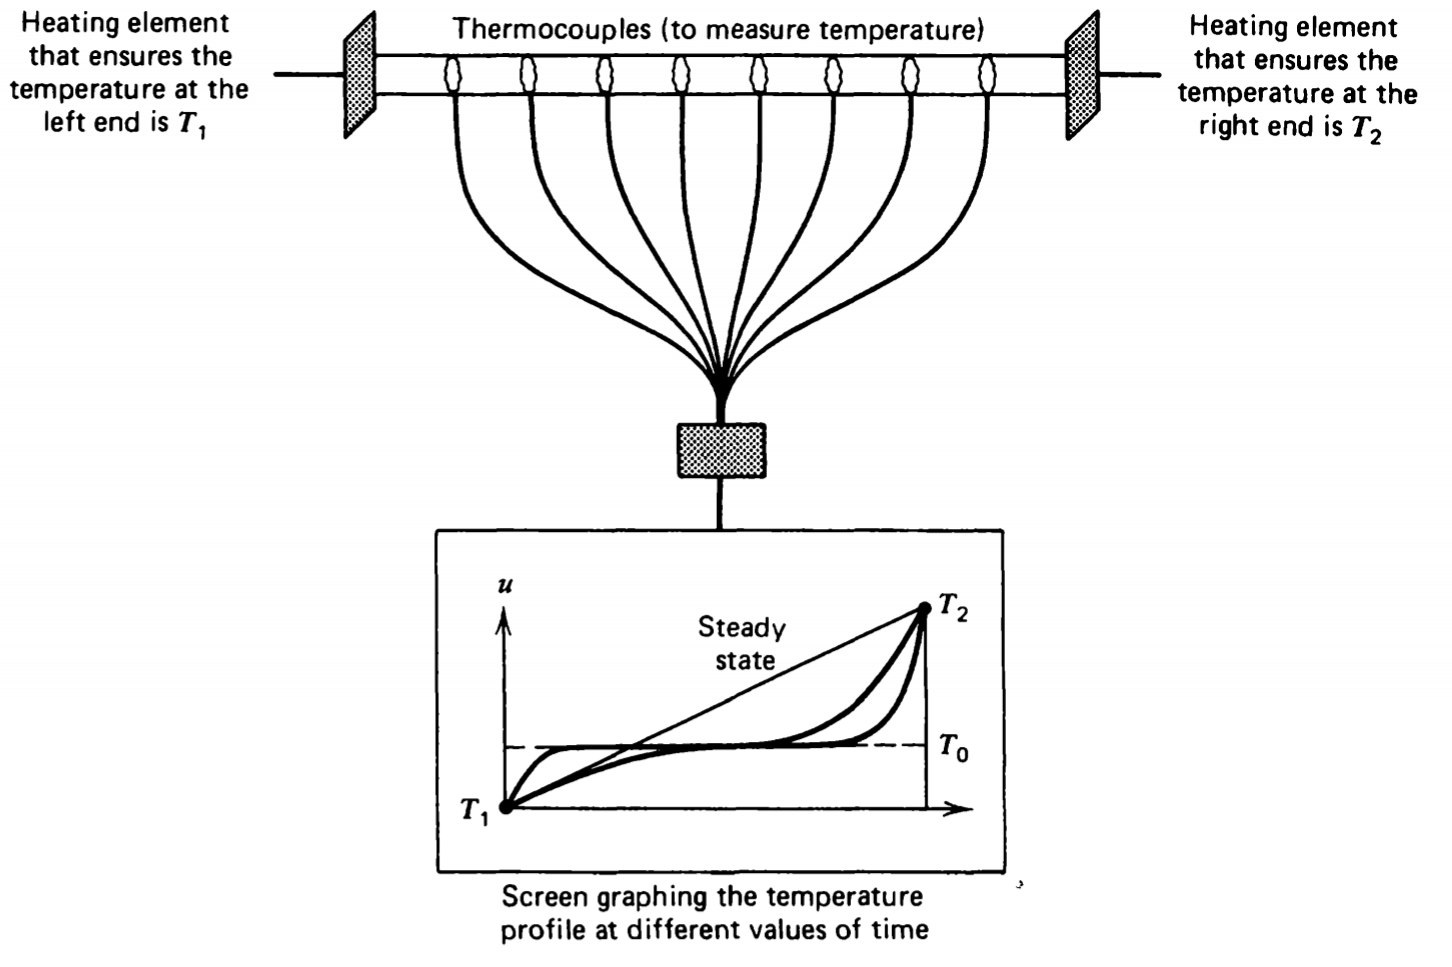
\includegraphics[scale=0.5]{copper.png}
\end{figure}

At time $t=0$, the temperature in the rod is known.
\begin{align*}
u(0,x) = T_0
\end{align*}
The ends of the rod are placed in thermal baths which hold their temperatures fixed. So, at $x=0$, $u(t,0) = T_1$ and at $x=L$, $u(t,L) = T_2$ for all $t>0$.
\subsection{The Mathematical Model}
This behavior is modeled by the heat equation. 
\begin{align*}
u_t = \alpha^2 u_{xx},
\end{align*}
where $\alpha \in \mathbb{R}$, determined by the thermo-character of the rod. $u_t$ is the rate of change of temperature in time, and $u_{xx}$ is the concavity profile in space. \\

Some justification for the heat equation: we look at the spatial difference quotient. For small change in $x$, $\Delta x$:
\begin{align*}
u_{xx} &\approx \frac{u_x(t,x+\Delta x) - u_x(t,x)}{\Delta x}\\
&\approx \frac{(u(t,x+\Delta x) - u(t,x))/\Delta x - (u(t,x)-u(t,x-\Delta x))/\Delta x}{\Delta x}\\
&\approx \frac{1}{\Delta x^2}(u(t,x+\Delta x) + u(t,x-\Delta x) - 2u(t,x))\\
&\approx \frac{2}{\Delta x^2}\left(\frac{u(t,x+\Delta x) + u(t,x-\Delta x)}{2} - u(t,x) \right)
\end{align*}
So, $u_{xx} \propto$ the difference between the average temperatures among neighboring points and the temperature at $x$. 
\begin{figure}[h!]
	\centering
	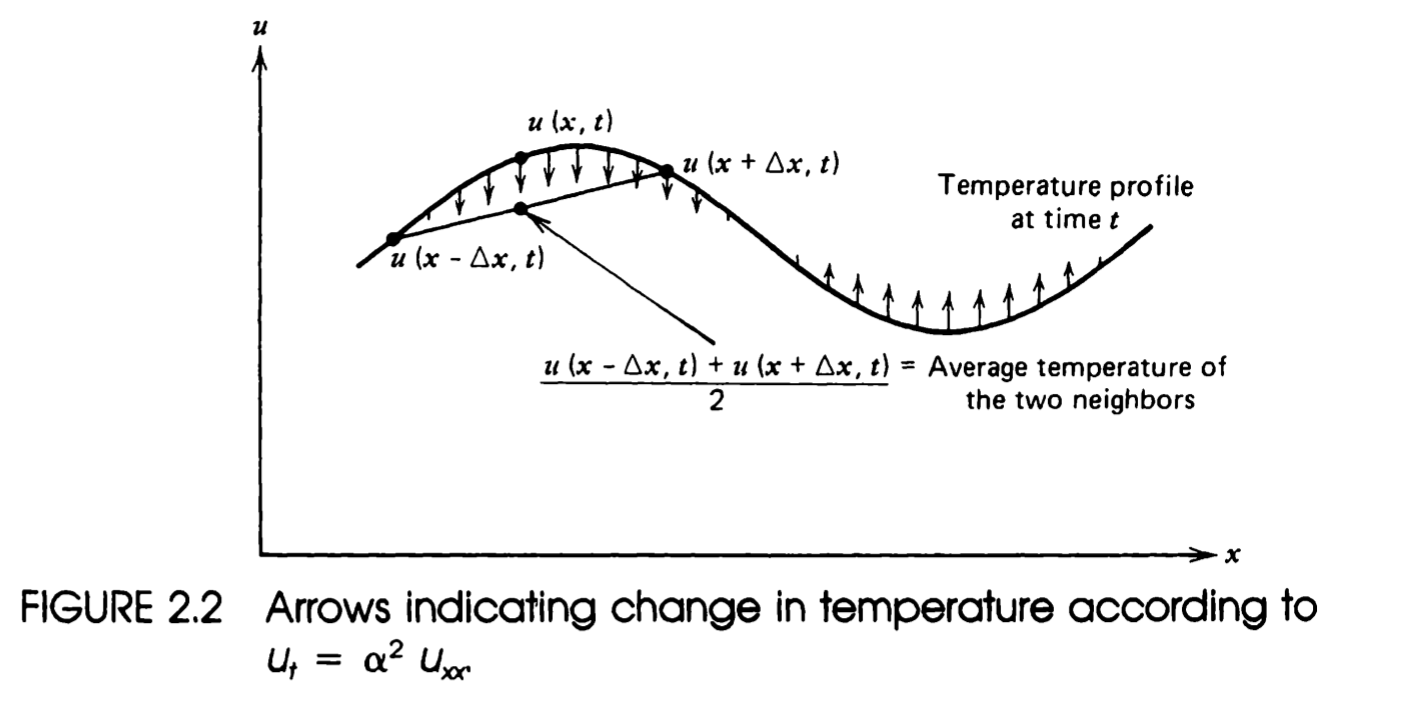
\includegraphics[scale=0.5]{copper1.png}
\end{figure}

Assume that $u_t = \alpha^2 u_{xx}$, then if $u_{xx} < 0$, then $u_t < 0$, i.e. temperature decreases in time. If $u_{xx} > 0$, then $u_t > 0$, i.e. temperature increases in time. If $u_{xx} = 0$, the temperature stays fixed. 

% Feb 11, 2019
\subsection{Boundary Conditions}
In contrast to ODEs, PDE have different types of constraints which are combined with the PDE to form well-posed problems, where ``well-posed'' means that a unique solution exists. Our conditions are often (and will almost always) be physically motivated. \\

Let us revisit the heat equation. 
\begin{align*}
u_t = \alpha^2 u_{xx}, t> 0, 0\leq x\leq L.
\end{align*}
The temperatures at the ends $x=0$ and $x=L$ are fixed $T_1$ and $T_2$ by the thermal baths, so the boundary conditions are
\begin{align*}
BCs = \begin{cases*}
u(0,t) = T_1\\
u(L,t) = T_2
\end{cases*}
\forall t > 0.
\end{align*} 
Here ``boundary'' refers to the boundary of $[0,L]$.
\subsection{Initial Conditions}
Our problem also involves evolution in time, we have an initial condition of the form
\begin{align*}
u(x,0) = T_0 \text{ or } u(x,0) = u_0(x) \forall x \in [0,L]
\end{align*}
where $T_0$ is the initial constant temperature of the rod and $u_0(x)$ is the initial temperature which is allowed to vary (some spatial distribution). All together, we form an initial boundary value problem, an IBVP of the form
\begin{align*}
\begin{cases*}
u_t = \alpha^2 u_{xx}, t>0,x\in[0,L]\\
u(0,t) = T_1, \forall t > 0\\
u(L,t) = T_2,\forall t > 0\\
u(x,0) = T_0, \forall x\in[0,L]
\end{cases*} 
\end{align*}
\subsection{A Couple of Variants}
\subsubsection{Lateral Heat Loss}
This allows for heat to be transferred laterally into the rod according to Newton's law of cooling. So the new heat equation is
\begin{align*}
u_t = \alpha^2 u_{xx} -\beta(u - u_0), \beta > 0
\end{align*}
where $u_0$ is the outside temperature.
\subsubsection{Internal Heat Source}
If, by some non-diffusive heat source, heat is added into the rod at $(t,x)$, the equation is
\begin{align*}
u_t = \alpha^2 u_{xx} + f(x,t)
\end{align*}
where $f(x,t)$ is the heat added to the rod, internally. This PDE is \textit{inhomogeneous}.
\subsubsection{Diffusion-convection Equation}
\begin{align*}
u_t = \alpha^2 u_{xx} - vu_x
\end{align*}
If $u$ describes the amount (not heat) pollutant, then the term $-vu_x$ describes the flow of additional pollutant introduced by the moving particles. 
\subsubsection{Variable-coefficients case}
When the thermal make up of the rod (its thermal character) is allowed to vary according to a variable diffusivity coefficient, i.e. $\alpha \rightarrow \alpha(x)$, then the relevant heat equation is
\begin{align*}
u_t = \alpha^2(x)u_{xx}.
\end{align*}
So, let's say
\begin{align*}
\alpha(x) = 
\begin{cases*}
\alpha_{Copper}, x\in[0,L/2]\\
\alpha_{Bronze}, x\in[L/2,L]
\end{cases*}
\end{align*}
\newpage
\section{Other types of Boundary Conditions}
\subsection{Type 1}
Let's revisit the original heat equation: $u_t = \alpha^2 u_{xx}$. If we force the rod ends to have time-dependent temperatures: $g_1(t)$ and $g_2(t)$ at $x=0$ and $x=L$ respectively, then our boundary conditions are
\begin{align*}
BCs = 
\begin{cases*}
u(0,t) = g_1(t)\\
u(L,t) = g_2(t)
\end{cases*}
\forall t > 0.
\end{align*} 
If instead we're studying the heat flow on a circular plate, i.e., where $u = u(t,t,\theta)$, and the heat EQ is 
\begin{align*}
u_t = \alpha^2 \nabla^2 u = \alpha^2\left( u_{rr} + \frac{1}{r}u_r + \frac{1}{r^2}u_{\theta\theta} \right).
\end{align*}
Here, the boundary conditions look like $u(t,r_0,\theta) = g(t,\theta)$, i.e. we force the disk to have temperature $g(t,\theta)$ along the boundary.
\subsection{Type 2 (more realistic)}
We take into account heat transfer to rod ends via thermal bath. Suppose that our rod is placed in bath (liquid) at each end of temperature $g_1(t)$ and $g_2(t)$ respectively. 
\begin{figure}[h!]
	\centering
	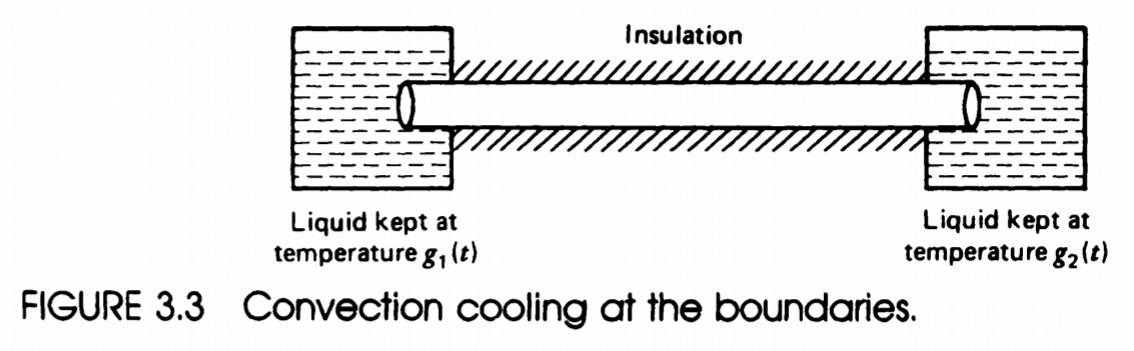
\includegraphics[scale=0.7]{type2.png}
\end{figure}

In view of Newton's law of cooling, the heat flux at a rod end is $h(u(t,0) - g_(1))$ at $x=0$ and $h(u(t,L)-g_2(t))$ at $x=L$, and $h$ is some constant. Next, we introduce Fourier's law of heat flux (empirical):
\begin{align*}
\frac{\p u}{\p n} = k \times\text{Heat flux}
\end{align*}
where $n$ is the \textit{inward normal} direction to the boundary, and $k\in\R$. At $x=0$:
\begin{align*}
\begin{cases*}
\frac{\p u}{\p n} = u_x(t,0) = kh(u(t,0)-g_1(t)), x=0\\
\frac{\p u}{\p n} = -u_x(t,L) = kh(u(t,L)-g_2(t)), x=L
\end{cases*}.
\end{align*}
So, the BC for Type 2 is the following
\begin{align*}
\begin{cases*}
u_x(t,0) = kh(u(t,0) - g_1(t))\\
u_2(t,L) = -kh(u(t,L) - g_2(t))
\end{cases*}
\end{align*}
The 2-D plate analogue is the following. We require (since $r$ is outward)
\begin{align*}
-\frac{\p u}{\p r} = -kh(u(t,r_0,\theta) - g(t,\theta))
\end{align*}
where $g(t,\theta)$ is the temperature of the bath surrounding the plate. 


\subsection{Type 3: Flux specified - including isolated boundaries} 
The rod ends are insulated, i.e., no heat flows in or out of the rod ends. So the boundary conditions are
\begin{align*}
u_x(0,t) = u_x(L,t) = 0 \forall 0 < t < \infty.
\end{align*}
In two variables (a disk), the analogous BC is
\begin{align*}
u_r(t,r_0,\theta) = 0 \forall 0 < t < \infty, 0\leq \theta \leq 2\pi.
\end{align*}
\subsection{Type 4: Mixed}
We can mix BCs. Suppose that one end of the rod has zero flux condition (type 3) and the other end is submerged in a liquid (type 2).

\begin{figure}[h!]
	\centering
	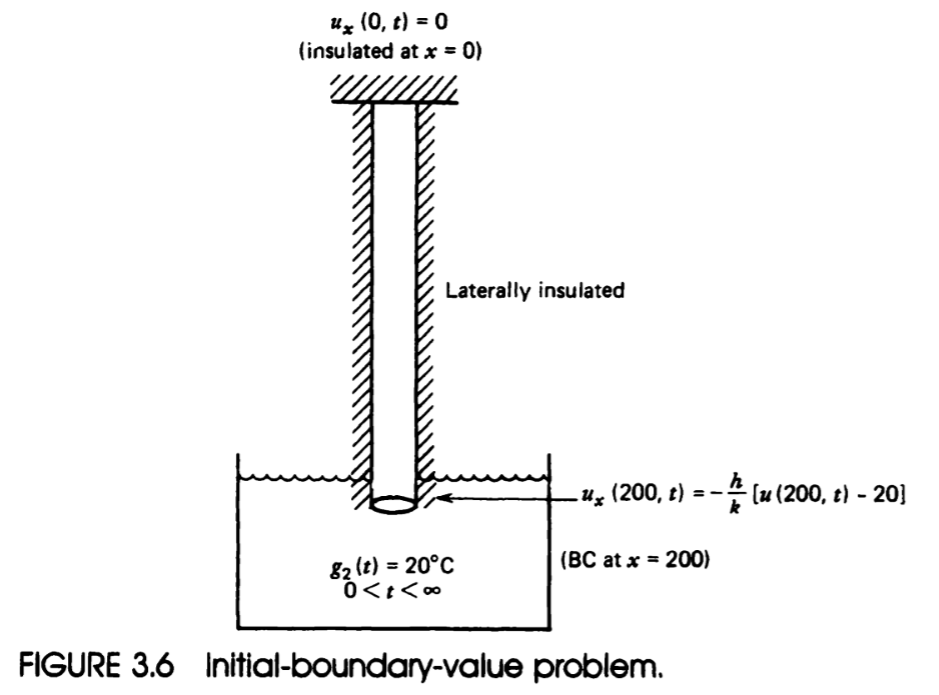
\includegraphics[scale=0.7]{type4.png}
\end{figure}

So, the IBVP is
\begin{align*}
\begin{cases*}
u_t = \alpha^2 u_xx\\
u_x(t,L) = 0\\
u_x(t,0) = -\lambda(u(t) - g_1(t)) \forall t > 0\\
u(0,x) = u_0(x) \forall 0\leq x \leq L
\end{cases*}
\end{align*}
\newpage
\section{Derivation of the Heat Equation}
\begin{figure}[h!]
	\centering
	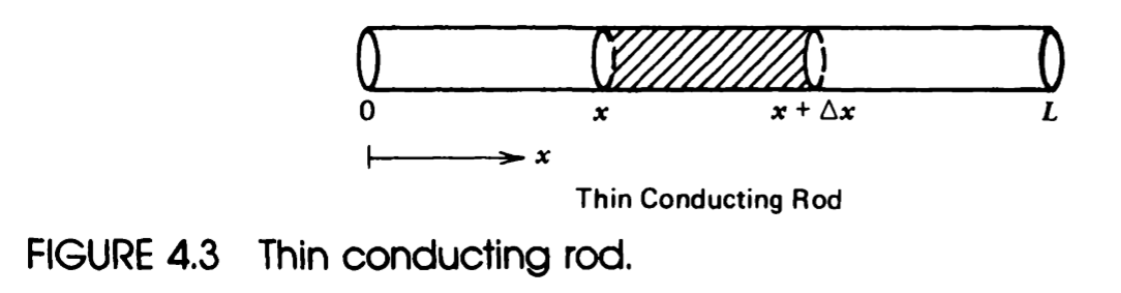
\includegraphics[scale=0.3]{heat.png}
\end{figure}
Main idea: Conservation of (Heat) Energy. Assumptions:
\begin{enumerate}
	\item The rod is a thermally homogeneous material 
	\item The temperature is constant across all cross-sections
	\item The rod is laterally insulated (no heat loss laterally)
\end{enumerate}
Using conservation of energy, we have the following: the change in thermal energy in the cross section $x$ to $x+\Delta x$ should be equal to the flux of the heat through the ``ends'' at $x$ and $x+\Delta x$ plus any external heat produced by some source (e.g. heat element). Some physical constants:
\begin{enumerate}
	\item $C$: thermal capacity of the rod
	\item $\rho$: density of the material of the rod
	\item $A$: area of cross section
	\item $k$: thermal conductivity
\end{enumerate}
Total heat inside is
\begin{align*}
\int_{x}^{\Delta x + x}c\rho A u(s,t)\,ds.
\end{align*}
The flux through the ends is
\begin{align*}
kA(u_x(x+\Delta x,t) - u_x(x, t)).
\end{align*}
The external energy is
\begin{align*}
A\int_x^{x+\Delta x}f(t,s)\,ds
\end{align*}
where $f(t,s)$ is the energy added at time $t$ and $x\leq s \leq x+\Delta x$. All together
\begin{align*}
\frac{d}{dt}\int_{x}^{\Delta x + x}c\rho A u(s,t)\,ds = kA(u_x(x+\Delta x,t) - u_x(x, t)) + A\int_x^{x+\Delta x}f(t,s)\,ds.
\end{align*}
Assuming that $u$ is nice enough, that
\begin{align*}
\frac{d}{dt}\int_{x}^{\Delta x + x}c\rho A u(s,t)\,ds = \int_{x}^{\Delta x + x}c\rho A u_t(s,t)\,ds.
\end{align*}
Also, the MVT for integrals says that if $G$ is continuous on the interval $[a,b]$ then $\exists c\in[a,b]$ such that
\begin{align*}
\int_a^b G(s)\,ds = G(c)(b-a).
\end{align*}
Therefore $\exists \chi \in [x,\Delta x]$ such that
\begin{align*}
\int_{x}^{\Delta x + x}c\rho A u_t(s,t)\,ds = c\rho A u_t(t,\chi)\Delta x
\end{align*}
and $\exists \eta \in [x,\Delta x]$ such that
\begin{align*}
A\int_x^{x+\Delta x}f(t,s)\,ds = Af(t,\eta)\Delta x.
\end{align*}
Combining all of these gives $\forall t > 0, \exists \chi,\eta \in [x,\Delta x]$ such that
\begin{align*}
c\rho Au_t(t,\chi)\Delta x &= kA(u_x(t,x+\Delta x) - u_x(t,x)) + Af(t,\eta)\Delta x\\
u_t(t,\chi) &= \frac{k}{\rho c}\frac{u_x(t,x+\Delta x) - u_x(t,x)}{\Delta x} + \frac{1}{c\rho}f(t,\eta).
\end{align*}
As $\Delta x \rightarrow 0$, $\eta,\chi \rightarrow x$
\begin{align*}
u_t(t,x) &= \frac{k}{\rho c}u_{xx}(x,t) + \frac{1}{c\rho}f(t,x)\\
u_t(t,x) &= \frac{k}{\rho c}u_{xx}(x,t) + F(t,x)\\
u_t(t,x) &= \alpha^2 u_{xx}(x,t) + F(t,x),
\end{align*}
where
\begin{align*}
\alpha^2 &= \frac{k}{\rho c}\\
F(t,x) &= \frac{1}{c\rho}f(t,x).
\end{align*}
\newpage
\section{Separation of Variables - First method of solution}
Main idea: If the IBVP is posed on a rectangle, e.g. $t>0,x\in[0,L]$, and the PDE is linear, it is often the case that this method reduces the PDE into ODEs. 
\subsection{Example: The heat equation}
\begin{align*}
u_t = \alpha^2 u_{xx}, t>0, x\in[0,1]
\end{align*}
We shall accompany this with so-called linear homogeneous BCs:
\begin{align*}
\alpha u(t,0) + \beta u_x(t,0) = 0\\
\gamma u(t,1) + \delta u_x(t,1) = 0.
\end{align*}
In fact, we specify further to assume
\begin{align*}
u(t,0)=0=u(t,1)\forall t > 0.
\end{align*}
We make an ansatz that solutions are of the form
\begin{align*}
u(t,x) = T(t)X(x).
\end{align*}
(Maybe not solutions but builidng blocks of solutions). Plug into the PDE, we get
\begin{align*}
u_t(t,x) = T'(t)X(x) = \alpha^2\p_x^2(u(t,x)) = \alpha^2 T(t)X''(x). 
\end{align*}
Separating variables gives
\begin{align*}
\frac{T'(t)}{\alpha^2 T(t)} = \frac{X''(x)}{X(x)} \forall t>0, x\in[0,1].
\end{align*} 
For this equation to hold for all independent $t$ and $x$, we must have that 
\begin{align*}
\frac{T'(t)}{\alpha^2 T(t)} = \frac{X''(x)}{X(x)} = \text{Const} \forall t>0, x\in[0,1].
\end{align*}
This immediately gives two ODEs connected by a constant $k$:
\begin{align*}
\begin{cases}
T(t) = \alpha^2 k T(t)\\
X''(x) = kX(x)
\end{cases}.
\end{align*}
By solving these equations, we hope to learn something aboaut $k$. The solution to the first solution is obvious:
\begin{align*}
K(t) = Ae^{\alpha^2 kt} \forall t > 0. 
\end{align*}
For physically reasonable solutions, we expect that the limit as $t\to \infty$ of $u(t,x) = 0$ and so, $T(t)\not\to\infty$ as $t\to\infty$, this forces $k<0$. Thus, we write $k=-\lambda^2$, $\lambda\in\R$, and denote
\begin{align*}
u_\lambda(t,x) = T(t)X(x) = X(x)Ae^{-\alpha^2\lambda^2t}.
\end{align*}
Next, the spatial ODE gives
\begin{align*}
X''(x) + \lambda^2 X(x) = 0.
\end{align*}
A general solution for this equation is
\begin{align*}
X(x) = A\sin(\lambda x) + B\cos(\lambda x).
\end{align*}
By absorbing multiplcative constants
\begin{align*}
u_\lambda(t,x) = e^{-\alpha^2\lambda^2 t}\left(A\sin(\lambda x) + B\cos(\lambda x) \right).
\end{align*}
Though we still don't know what $\lambda$ is, let us force this solution to satisfy the boundary conditions to learn more. Since the boundary conditions require that $u(t,0)=0=u(t,1)$, we require that
\begin{align*}
\begin{cases}
B=0\\
\lambda = \pm n\pi
\end{cases}
\end{align*}
where $n\in \mathbb{N}$, for non-trivial solutions (where $A\neq 0$). Thus, with separation of variables, we find that
\begin{align*}
u_n(t,x) = A_ne^{-(n\alpha\pi)^2}\sin(n\pi x).
\end{align*}
This is a solution for any $n\in \mathbb{N}$ and $A_n\in\R$. Just to be sure that we haven't made an error, we can readily verify this solution. This is left as an exercise to the reader. \\

Note that we still have some ``degrees of freedom'' - $A_n$ and $n$. So, we have established the existence of \textit{many} solutions, for each $n\in\mathbb{N}$ and $A_n\in\R$. Now, we make use of the principle of superposition to generate more solutions. The principle of superposition (works for linear DEs) says that all convergent sums of solutions are solutions. More generally, for any collection $\{A_n \} \subseteq\R$,
\begin{align*}
u(t,x) = \sum_{n=1}^\infty A_n e^{-(n\pi\alpha)^2}\sin(n\pi x)
\end{align*}
is also a solution. But divergence could be a problem here. It might be that $u(t,x)$ fails to exist, or differentiation might not work. But worry not, since the presence of the term $e^{-(n\pi\alpha)^2}$ makes this series always converge. And so, we have that for any sequence $\{ A_n\}$, $u(t,x)$ defined in this way solves the DE $u_t = \alpha^2 u_{xx}$ and satisfies the boundary conditions $u(t,0)=0=u(t,1)$. The problem of satisfying the initial condition $u(0,x) = u_0$ becomes one of finding the ``right'' constants $A_n$ so that 
\begin{align*}
u(0,x) = \sum_{n=1}^\infty A_n\sin(n\pi x) = u_0(x).
\end{align*} 

% feb 18, 2019} 
The term on the left hand side is called the trigonometric series. The question now becomes whether it is possible to find the sequence $\{ A_n\} \subseteq \R$ so that
\begin{align*}
u(0,x) = \sum_{n=1}^\infty A_n \sin (n \pi x) = u_0(x).
\end{align*}
Another question would be which function $u_0(x)$ can be expanded as a trigonometric series as above.

\begin{exmp}
	Consider
	\begin{align*}
	u_0(x) = \frac{1}{2}\sin(2\pi x) + \frac{1}{50}\sin(201\pi x).
	\end{align*}
	We see that
	\begin{align*}
	A_n = 0, A_2 = \frac{1}{2}, A_{201} = \frac{1}{50} \forall n\neq 2,201.
	\end{align*}
\end{exmp}

\begin{exmp}
	What about
	\begin{align*}
	u_0(x) = \begin{cases}
	x, 0\leq x < \frac{1}{2}\\
	1-x, \frac{1}{2} < x \leq 1
	\end{cases}
	\end{align*}
	or
	\begin{align*}
	u_0(x) = 1?
	\end{align*}
\end{exmp}


It's clear that we must have that $u_0(0) = u_1(1) = 0$, otherwise this cannot be done. To treat otherwise, one needs a cosine term. But what if $u_0(0) = u_0(1) = 0$, but $u_0(x)$ is very bad? Suppose that this can be done. Using the property that 
\begin{align*}
\int_{0}^1 \sin(n\pi x)\sin(m\pi x) = \frac{1}{2}\delta^m_n,
\end{align*}
we use \textbf{Fourier's trick}: multiply both sides of the $u_0(x)$ expansion by $\sin(m \pi x)$ and integrate:
\begin{align*}
\int^1_0 u_0(x)\sin(m \pi x) &= \sum_{n=1}^\infty\int_{0}^1A_n\sin(n\pi x)\sin(m \pi x)\,dx\\
&= \sum_{n=1}^\infty A_m\frac{1}{2}\delta^m_n.
\end{align*}
So this gives
\begin{align*}
A_m = 2\int^1_0 u_0(x)\sin(m\pi x)\,dx \forall m\in \mathbb{N}.
\end{align*}
This gives a prescription for finding the sequence $\{A_m \}$ so that the expansion works. So, we might ask, given a function $u_0(x)$ with value 0 at $x=0,1$ and define
\begin{align*}
A_m = 2\int^1_0 u_0(x)\sin(m\pi x)\,dx\,\,\, \forall m\in \mathbb{N},
\end{align*}
when does 
\begin{align*}
u_0(x) = \sum^\infty_{n=1}A_n \sin(n\pi x)?
\end{align*}
Usually, this works perfectly, but around 1802, the mathematician DuBois Reymond found an example for which the \textbf{Fourier series} does not hold. The exact class of such functions was determined explicitly in 1962 by UCLA professor L. Carelson. The answer is $L^2[0,1]$ - square integrable functions. \\

\begin{exmp}
	Now, let's find $A_n$ so that 
	\begin{align*}
	u_0(x) = \begin{cases}
	x, 0\leq x < \frac{1}{2}\\
	1-x, \frac{1}{2} < x \leq 1
	\end{cases}.
	\end{align*}
	Well,
	\begin{align*}
	A_n &= 2\int_{0}^1 u_0(x)\sin(n\pi x)\,dx = 2\int_{0}^\frac{1}{2} x\sin(n\pi x)\,dx + 2\int_{\frac{1}{2}}^1 (1-x)\sin(n\pi x)\,dx\\
	&= 2\int_{0}^\frac{1}{2} x\sin(n\pi x)\,dx - 2\int_\frac{1}{2}^1 +  x\sin(n\pi x)\,dx + 2\int_{\frac{1}{2}}^1 \sin(n\pi x)\,dx
	\end{align*}
	Integration by parts...
	\begin{align*}
	\int x\sin(kx)\,dx = \frac{-1}{k}x\cos(kx) - \int \frac{-\cos(kx)}{k}\,dx = \frac{1}{k^2}\sin(kx) - \frac{x\cos(kx)}{k}.
	\end{align*}
	So
	\begin{align*}
	2\left( \frac{1}{(n\pi)^2}\sin(n\pi x) - \frac{x}{\pi n}\cos(n\pi x)
	 \right)\bigg\vert^{1/2}_0
	 = \frac{2}{(n\pi)^2}\sin\left( \frac{n\pi}{2}\right)  - \frac{1}{n\pi}\cos\left( \frac{n\pi}{2}\right).
	\end{align*}
	\begin{align*}
	2\int_{\frac{1}{2}}^1 (1-x)\sin(n\pi x)\,dx = 
	\frac{2}{n\pi}\left( \cos\left(\frac{n\pi}{2} \right)  - \cos(n\pi)\right).
	\end{align*}
	\begin{align*}
	2\int_\frac{1}{2}^1 x\sin(n\pi x)\,dx = \frac{2}{n\pi}\cos(n\pi) - \frac{2}{(n\pi)^2}\sin\left( \frac{n\pi}{2} \right) + \frac{1}{n\pi}\cos\left(\frac{n\pi}{2} \right).
	\end{align*}
	So, all together,
	\begin{align*}
	A_n = \frac{4}{(n\pi)^2}\sin\left( \frac{n\pi}{2}\right).
	\end{align*}
	So our series is
	\begin{align*}
	u_0(x) = \sum_{n=1}^\infty \frac{4}{(n\pi)^2}\sin\left( \frac{n\pi}{2}\right) \sin(n\pi x)
	\end{align*}
	This converges nicely. 
\end{exmp}

Recap: to solve our IVBP, we defines 
\begin{align*}
A_n = 2\int_{0}^1 u_0(x)\sin(n\pi x)\,dx, \,\,\, n\in \mathbb{N}
\end{align*}
and then (provided that things converge nicely)
\begin{align*}
u(t,x) = \sum_{n=1}^\infty A_n e^{-(\alpha \pi n)^2 t}\sin(n\pi x)
\end{align*}
is \textbf{the} solution. More generally, on the interval $[0,L]$ for the same IVBP with $u(t,0) = u(t,L) = 0$ and $u(0,x) = u_0(x), x\in[0,L]$, then the solution is given by
\begin{align*}
u(t,x) = \sum_{n=1}^\infty A_n e^{-(\alpha \pi n/L)^2 t}\sin\left(\frac{n\pi x}{L}\right)
\end{align*}
where 
\begin{align*}
A_n = \frac{2}{L}\int_{0}^1 u_0(x)\sin\left(\frac{n\pi x}{L}\right)\,dx, \,\,\, n\in \mathbb{N}.
\end{align*}
One more note: as $t\to \infty$, the solution is dominated lower order terms
\begin{align*}
u(t,x)\approx A_1 e^{-(\alpha \pi/L)^2 t}\sin\left(\frac{\pi x}{L}\right).
\end{align*}





\newpage
\section{Transforming Nonhomogeneous Boundary Conditions into Homogeneous ones }

\subsection{Inhomogeneous BCs to Homogeneous Ones}

Question: how can we solve inhomogeneous BCS? Given $k_1,k_2\in\R$ and $u_0(x)$, can we solve
\begin{align*}
\begin{cases}
u_t = \alpha^2u_{xx}\\
u(t,0) = k_1\\
u(t,L) = k_2\\
u(0,x) = u_0(x)
\end{cases}
\end{align*}

Idea: in the steady-state, we expecet that $u_t = 0$, so $u(x,t) \to u(x) = Cx+D$. So, the steady state is
\begin{align*}
S(t,x) = k_1\left( 1 - \frac{x}{L} \right) + k_2\left(\frac{x}{L} \right).
\end{align*}
To solve the problem, we assume 
\begin{align*}
u(t,x) = S(t,x) + U(t,x)
\end{align*}
where $S(t,x)$ is the steady-state solution, and $U(t,x)$ is the transient solution. Let's plug $u = S+U$ into our problem to learn something about $U$. First, 

\begin{align*}
u_t = S_t + U_t &= \alpha^2 (S_{xx} + U_{xx})\\
U_t &= \alpha^2 U_{xx}.
\end{align*}
Using the BCs in out IBVP,
\begin{align*}
k_1 = u(t,0) = S(t,0) + U(t,0) = k_1 + U(t,0).
\end{align*}
So
\begin{align*}
U(t,0) = 0.
\end{align*}
And similarly,
\begin{align*}
U(t,L) = 0.
\end{align*}
Finally, 
\begin{align*}
u_0(x) = u(0,x) = S(0,x) + U(0,x)
\end{align*}
and hence
\begin{align*}
U(0,x) = u_0(x) - S(0,x).
\end{align*}
So, summary: $u(t,x)$ satisfies the IBVP $\iff$ 
\begin{align*}
u(t,x)=S(t,x)+U(t,x) = k_1\left( 1 - \frac{x}{L} \right) + k_2\left(\frac{x}{L} \right) + U(t,x)
\end{align*}
where $U(t,x)$ solves the auxiliary IBVP:


\begin{align*}
\begin{cases}
U_t = \alpha^2U_{xx}\,\,\,\, t>0,0<x<L\\
U(t,0) = 0\,\,\, t> 0\\
U(t,L) = 0\\
U(0,x) = u_0(x) - S(0,x)\,\,\,\,\, x\in[0,L]
\end{cases},
\end{align*}
which we know how to solve using separation of variables and Fourier series. 

\subsection{Time Varying BCs into Zero BCs}
\begin{align*}
\begin{cases}
u_t = \alpha^2u_{xx}\,\,\,\,, t>0,0<x<L\\
\alpha_1 u(t,0) + \beta_1 u_x(t,0) = g_1(t)\\
\alpha_2 u(t,L) + \beta_2 u_x(t,L) = g_2(t)\\
u(0,x) = u_0(x)\,\,\,\,\,, x\in[0,L]
\end{cases},
\end{align*}
where $\alpha_1,\alpha_2,\beta_1,\beta_2,g_1(t),g_2(t),u_0(x)$ are all known. To solve this, we push forwardour idea of steady-state-ish and transient solutions. We assume that 
\begin{align*}
u(t,x)= S(t,x) + U(t,x)
\end{align*}
where
\begin{align*}
S(t,x) = A(t)\left( 1 - \frac{x}{L}\right) + B(t)\frac{x}{L}
\end{align*}
Can we find $A(t)$ and $B(t)$ in terms of $\alpha_1,\alpha_2,\beta_1,\beta_2,g_1(t),g_2(t),u_0(x)$? We want to choose $S(t,x)$ so that it absorbs all of the \textit{complicated} nature of the BCs for $u(t,x)$. So, we can make $S$ satisfy $u's$ BCs. 
\begin{align*}
S(t,0)&= A(t)\\
S_x(t,0) &= \frac{B(t) - A(t)}{L}  = S_x(t,L)\\
S(t,L) &= B(t).
\end{align*}
So we have
\begin{align*}
\alpha_1 S(t,0) + \beta_1 S_x(t,0) &= g_1(t)\\
\alpha_1 A(t) + \frac{\beta_1(B(t) - A(t))}{L} &= g_1(t)
\end{align*}
and
\begin{align*}
\alpha_2 S(t,L) = \beta_2 S_x(t,L) &= g_2(t)\\
\alpha_2 B(t) + \frac{\beta_2(B(t) - A(t))}{L} &= g_2(t).
\end{align*}
Rewriting gives
\begin{align*}
\Gamma\begin{pmatrix}
A(t)\\B(t)
\end{pmatrix} = 
\begin{pmatrix}
\alpha_1 - \frac{\beta_1}{L} & \frac{\beta_1}{L}\\
- \frac{\beta_2}{L} & \alpha_2  + \frac{\beta_2}{L}
\end{pmatrix}
\begin{pmatrix}
A(t)\\B(t)
\end{pmatrix}
=
\begin{pmatrix}
g_1(t)\\g_2(t)
\end{pmatrix}
\end{align*}
So
\begin{align*}
\begin{pmatrix}
A(t)\\B(t)
\end{pmatrix} = \Gamma^{-1}\begin{pmatrix}
g_1(t)\\g_2(t)
\end{pmatrix}=
\begin{pmatrix}
\rho_{11}(t)&\rho_{12}(t)\\
\rho_{21}(t) & \rho_{22}(t)
\end{pmatrix}
\begin{pmatrix}
g_1(t)\\g_2(t)
\end{pmatrix}
\end{align*}
Of course, this requires $\Gamma$ to be invertible, i.e, 
\begin{align*}
\det(\Gamma) = \left(\alpha_1 - \frac{\beta_1}{L}\right)\left(\alpha_2  + \frac{\beta_2}{L}\right) +  \frac{\beta_1}{L}\frac{\beta_2}{L} = \alpha_1 \alpha_2 + \frac{\alpha_1\beta_2}{L} - \frac{\alpha_2\beta_1}{L}\neq 0.
\end{align*}
Assuming this is true
\begin{align*}
S(t,x) = (\rho_{11}g_1(t) + \rho_{12}g_2(t))\left(1 - \frac{x}{L} \right) + (\rho_{21}g_1(t) + \rho_{22}g_2(t))\frac{x}{L}
\end{align*}
Now, let us see what this implies for $U$. 
\begin{align*}
u_t = S_t + U_t = U_t = \alpha^2(S_{xx} +  U_{xx}) = \alpha^2 U_{xx}.
\end{align*}
So, once again
\begin{align*}
U_t = \alpha^2 U_{xx} - S_t.
\end{align*}
Also, by an easy calculation, we have that $u$ satisfying the inhomogeneous BCs implies
\begin{align*}
U(t,0) = U(t,L) = 0.
\end{align*}
And further, that
\begin{align*}
U(0,x)= u_0 - S(0,x)
\end{align*}
is just a linear function of $x$. So, by setting 
\begin{align*}
S(t,x)= (\rho_{11}g_1(t) + \rho_{12}g_2(t))\left(1 - \frac{x}{L} \right) + (\rho_{21}g_1(t) + \rho_{22}g_2(t))\frac{x}{L},
\end{align*}
we see that
\begin{align*}
u(t,x) = U(t,x) + S(t,x)
\end{align*}
satisfies a IBVP where the heat equation is homogeneous, but the BCs are very complicated compared to the new inhomogeneous heat IBVP. 
\begin{align*}
\begin{cases}
U_t = \alpha^2 U_{xx} - S_t\\
U_x(L,t) = 0\\
U(t,L) = 0\\
U(0,x) = u_0(x) - S(0,x)
\end{cases}.
\end{align*}
Moral: problems with complicated BCs can often be transformed into equivalent problems with simple BCs at the cost of making the PDE more complicated. \\

Question: Under what conditions on the first IBVP is our new IBVP homogeneous? The answer is that a sufficient condition is for $g_1$, $g_2$ to be constant. In this realm, $S(t,x) = S(x)$ nad is thus a ``real'' steady-state solution.

\newpage

\section{Solving more complicated problems directly: An invitation to Strum-Liouville theory}

Consider the following IBVP:
\begin{align*}
\begin{cases}
u_t = \alpha^2 u_{xx}\\
u(t,0) = 0\\
u_x(t,1) + hu(t,1) = 0\\
u(0,x) = u_0(x) 
\end{cases}.
\end{align*}
We can solve this using separation of variables. First, we seek product solutions of the form:
\begin{align*}
u(t,x) = T(t)X(x).
\end{align*}
By asking that $u_t = \alpha^2 u_{xx}$, we obtained 
\begin{align*}
\frac{T'(t)}{\alpha^2 T(t)} = \frac{X''(x)}{X(x)} = \mu
\end{align*}
where $\mu$ is a constant. What are the possibilities for $\mu$?\\

\subsection{$\mu > 0$}
If $\mu>0$, we obtain
\begin{align*}
u(t,x) = Ae^{\alpha^2 \mu t}X(x).
\end{align*}
But as $e^{\alpha^2 \mu t} \to \infty$ as $t\to\infty$, we reject this solution on physical grounds. \\
\subsection{$\mu=0$}
If $\mu = 0$, then $T'(t) = X''(x) = 0$, so
\begin{align*}
u(t,x) = Ax+b.
\end{align*}

To satisfy the BCs in this case:
\begin{align*}
u(t,0) = 0 = A\times 0 + b.
\end{align*}
So, $b=0$. Next,
\begin{align*}
u_x(t,1) + hu(t,1) = 0.
\end{align*}
So, $A+hA = 0$, so $A=0$. This is just the trivial solution.

\subsection{$\mu <0$}
Let $\mu=\lambda^2$, then we have
\begin{align*}
T(t) = Ae^{-(\alpha \lambda)^2t}
\end{align*}
and
\begin{align*}
X(x) = A\sin(\lambda x) + B\cos(\lambda x).
\end{align*}
So,
\begin{align*}
u(t,x) = e^{-(\lambda\alpha)^2t}\left( A\sin(\lambda x) + B\cos(\lambda x) \right).
\end{align*}
We let this subject to BCs:
\begin{align*}
u(t,0) = e^{-(\lambda\alpha)^2t}\left( A\sin(\lambda\times 0) + B\cos(\lambda \times 0) \right) = 0.
\end{align*}
So, $B=0$. Thus our product solution looks like
\begin{align*}
u(t,x) = Ae^{-(\lambda\alpha)^2t}\sin(\lambda x).
\end{align*}
The other BC gives
\begin{align*}
0=u(t,1)+hu_x(t,1)=Ae^{-(\lambda\alpha)^2t}\left( \lambda\cos(\lambda) + h\sin(\lambda) \right).
\end{align*}
So,
\begin{align*}
\tan\lambda - \frac{-\lambda}{h}.
\end{align*}

So, admissible $\lambda$'s here are solution to this equation, which is not as simple as $\pi n$, like we have found before. Now, note that $\lambda$ is this equation cannot be found explicitly. Solutions are just intersections on the following plot:
\begin{figure}[h!]
	\centering
	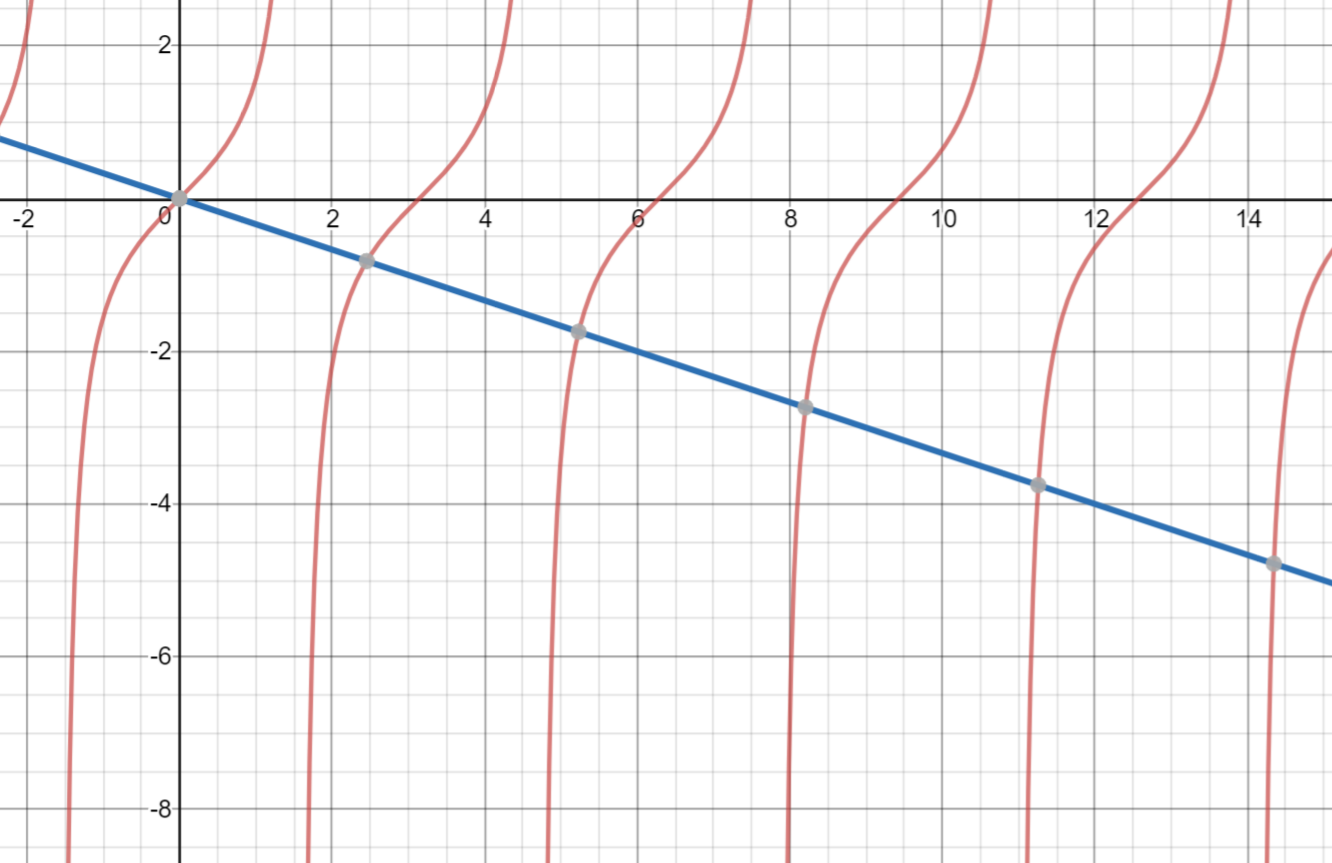
\includegraphics[scale=0.6]{tan.png}
\end{figure}

We see that
\begin{align*}
\frac{\pi}{2} < \lambda_1 < \pi < \lambda_2 < 2pi < \lambda_3 < 3\pi.
\end{align*}
We call these $\lambda_n$'s eigenvalues associated with the boundary value problem
\begin{align}
\begin{cases}
X'' + \lambda^2 X = 0\\
X(0) = 0\\
X'(1) + hX(1) = 0
\end{cases}.
\end{align}
The solutions, $\sin(\lambda_n x)$ are associated eigenfunction. So, with separation of variables, we obtain
\begin{align*}
u_n(x,t) = A_n e^{-(\lambda_n\alpha)^2t}\sin(\lambda_n x)
\end{align*}
which solve the IBVP. Once again, we have that
\begin{align*}
u(t,x) = \sum_{n=1}^{\infty} A_n e^{-(\lambda_n\alpha)^2t}\sin(\lambda_n x)
\end{align*}
which we want to also satisfy the IC, which is 
\begin{align*}
u(0,x) = u_0(x).
\end{align*}
We invoke Fourier's trick to find $A_n's$:
\begin{align*}
\int_{0}^1 u_0(x)\sin(\lambda_m x)\,dx &= \int_{0}^1 \sin(\lambda_m x)\sum_{n=1}^{\infty} A_n e^{-(\lambda_n\alpha)^2t}\sin(\lambda_n x)\,dx\\
&= \sum_{n=1}^\infty A_n\int_{0}^1 \sin(\lambda_m x)\sin(\lambda_n x)\,dx\\
&= A_m \left( \frac{1}{2} - \frac{\sin(2\lambda_m x)}{4\lambda_m} \right).
\end{align*}
So
\begin{align*}
\int_{0}^1 u_0(x)\sin(\lambda_m x) \,dx &= A_m \frac{1}{2\lambda_m}\left( \lambda_m - \sin(\lambda_m x)\cos(\lambda_m x) \right)
\end{align*}
and so
\begin{align*}
A_m = \frac{2\lambda_m}{\lambda_m - \sin(\lambda_m x)\cos(\lambda_m x)}\int_{0}^1 u_0(x)\sin(\lambda_m x) \,dx.
\end{align*}

\noindent Summary: Recall the IBVP:
\begin{align*}
\begin{cases}
u_t = \alpha^2 u_{xx}\\
u(t,0) = 0\\
u_x(t,1) + hu(t,1) = 0\\
u(0,x) = u_0(x) 
\end{cases}.
\end{align*}
In trying to solve it, we have found
\begin{align*}
u(t,x) \sum_{n=1}^{\infty}A_n e^{-(\alpha \lambda)^2t}\sin(\lambda_n x)
\end{align*}
to be a solution with
\begin{align*}
A_m = \frac{2\lambda_m}{\lambda_m - \sin(\lambda_m x)\cos(\lambda_m x)}\int_{0}^1 u_0(x)\sin(\lambda_m x) \,dx.
\end{align*}
where $\lambda_n$ is the n$^{th}$ positive solution to 
\begin{align*}
\frac{-\lambda}{n}= \tan(\lambda)
\end{align*}
Question: In our finding of $A_n$, we swept a detail under the rug. It was \textbf{orthogonality}. We assumed the fact that for all $n,m$
\begin{align*}
\int^1_0 \sin(\lambda_m x)\sin(\lambda_n x)\,dx = 0,\,\,\,\,\,\,\text{ if } m\neq n.
\end{align*}
This would be obvious if $\lambda_n = n\pi$. But it is not the case here. We will look at this in the next section.
\newpage
\section{ODE Boundary Value Problems - a look at the Sturm-Liouville theory}
(reference: Boyce-DiPrima, Chapter 11).\\


Motivating example:
\begin{align*}
\begin{cases}
ODE: y'' + \lambda y = 0\\
BC: y(0) = y(1) = 0, 0\leq x\leq 1.
\end{cases}.
\end{align*}
We ask: does solving this BVP require anything about $\lambda$? Is it possible to find non-zero solutions to this problem for arbitrary $\lambda$? We can try...\\

If $\lambda = 0$, then $y(x) = Ax+B$. By subjecting to the BCs, we get $A=B=0$. So, not every $\lambda$ gives a non-trivial solution. This $\lambda$ does not admit non-zero solutions. This is in stark contrast to IVP which can be solved for any non-zero $\lambda$.\\

If $\lambda < 0$, we get the same issue (can check that there are no non-zero solutions for $\lambda< 0$. \\

If $\lambda > 0$, then $y(x) = C_1 \sin(\sqrt{\lambda} x ) + C_2 \cos(\sqrt{\lambda} x)$. Subject to boundary conditions, we have $C_2 = 0$ and
\begin{align*}
C_1 = \sin(\sqrt{\lambda} x).
\end{align*}
For non-trivial solutions,
\begin{align*}
\sqrt{\lambda}=n\pi.
\end{align*}
Or for $n=1,2,3,\dots$
\begin{align*}
\lambda_n = n^2 \pi^2.
\end{align*}

The moral: Not every $\lambda$ works. So we ask: Given a linear ODE and linear homogeneous BCs, which $\lambda$ (if any) will work?\\

\begin{defn}
	\textbf{General theory:} Consider the ODE
	\begin{align*}
	(p(x)y')' - q(x)y + \lambda r(x)y = 0,
	\end{align*}
	where we will let $p,q,r \in C^0([0,1])$. Moreover, $p(x) \in C^1([0,1])$. Finally, $p(x),r(x) > 0$ for all $x\in[0,1]$. Also, consider the linear homogeneous BCs:
	\begin{align*}
	a_1y(0) + b_1y'(0) &= 0\\
	a_2y(1) + b_2y'(1) &= 0.
	\end{align*}
	
	If, for some fixed $\lambda$, the ODE and the BCs have a non-zero solution $\phi(x)$, we say that $\lambda$ is an \textbf{eigenvalue} for the BVP, and $\phi(x)$ is an \textbf{eigenfunction} corresponding to $\lambda$. \\
	
	An eigenvalue $\lambda$ corresponding to the BVP is said to be simple if it does not have two linearly independent eigenfunctions $\phi_1, \phi_2$. 
	\qed
\end{defn}

\begin{rmk}
	$\,$\\
	\begin{enumerate}
		\item We will write 
		\begin{align*}
		L[y] = -(p(x)y')' + q(x)y,
		\end{align*}
		which is a second-order linear operator. Then the ODE becomes:
		\begin{align*}
		L[y] = \lambda r(x)y.
		\end{align*}
		For this reason, we see the ``eigen'' terminology arises. 
	\end{enumerate}
\end{rmk}

Given our ODE, the theory of ODE gives, for fixed $\lambda$, two linearly independent solutions of the form $y_1 = y_1(x,\lambda), y_2 = y_2(x,\lambda)$, and so all solutions to the ODE is of the form
\begin{align*}
y(x) = C_1 y_1(x,\lambda) + C_2y_2(x,\lambda).
\end{align*}
Question: can we find a condition on $\lambda$ so that $y$ above is a non-zero solution satisfying the BCs? Sure we can. Let us subject $y$ to the BCs. We have
\begin{align*}
0 = a_1y(0) + b_1 y'(0) =& a_1(C_1y_1(0,\lambda) + C_2y_2(0,\lambda)) + b_1(C_1y'_1(0,\lambda) + C_2y'_2(0,\lambda))\\
&= C_1(a_1y_1(0,\lambda) + b_1y'_1(0,\lambda)) + C_2(a_1y_2(0,\lambda) + b_1y'_2(0,\lambda)).
\end{align*}
Similarly, 
\begin{align*}
0 = C_1(a_2y_1(1,\lambda) + b_2y'_1(1,\lambda)) + C_2(a_2y_2(1,\lambda) + b_2y'_2(1,\lambda)).
\end{align*}
As a matrix equation,
\begin{align*}
A\begin{pmatrix}
C_1\\C_2
\end{pmatrix}=
\begin{pmatrix}
0\\0
\end{pmatrix}=
\begin{pmatrix}
a_1y_1(0,\lambda) + b_1y'_1(0,\lambda) & a_1y_2(0,\lambda) + b_1 y'_2(0,\lambda)\\
a_2y_1(1,\lambda) + b_2y'_1(1,\lambda) & a_2y_2(1,\lambda) + b_2y'_2(1,\lambda)
\end{pmatrix}
\begin{pmatrix}
C_1\\C_2
\end{pmatrix}.
\end{align*}
To get non-trivial solution, we require that $\ker(A)\neq \{ 0\}$, i.e., $\det(A) = 0$. This gives a necessary and sufficient condition on $\lambda$, since $a_i,b_i$ and the solutions are known, that is
\begin{align*}
\boxed{\det(A)=0}
\end{align*}

% Feb 27, 2019 % 

Recall that $$ L[y] = -(p(x)y')' + q(x)y.$$ So the ODE is $$ L[y] = \lambda r(x) y.$$ 

\begin{prop}
	\textbf{Lagrange's Identity:} For any $u,v \in \mathbb{C}^2([0,1])$, the following identity holds:
	\begin{align*}
	\int^1_0 (uL[v] - vL[u])\,dx = p(x)\left( u'(x)v(x) - u(x)v'(x) \right)\bigg\vert^1_0.
	\end{align*}
	Intuitively, this is essentially an integration by parts formula for the operator $L$.
	
	
	\begin{proof}
		We have
		\begin{align*}
		u(x)L[v](x) - v(x)L[u](x) &= u(x)(-(p(x)v')' + q(x)v) - v(x)(-(p(x)u')' + q(x)u)\\
		&= -u(x)(p(x)v'(x))' + u(x)q(x)v(x) + v(x)(p(x)u(x))' - q(x)v(x)u(x)\\
		&= -u(x)(p(x)v'(x))' + v(x)(p(x)u(x))'.
		\end{align*}
		So the integral becomes
		\begin{align*}
		\int^1_0 (uL[v] - vL[u])\,dx &= \int^1_0 -u(x)(p(x)v'(x))' + v(x)(p(x)u(x))'\,dx\\
		&= \int^1_0 -u(x)(p(x)v'(x))' \,dx    + \int^1_0 v(x)(p(x)u(x))' \,dx\\
		&= -u(x)(p(x)v'(x))\bigg\vert^1_0 - int^1_0 -u'(x)p(x)v'(x)\,dx +\\ v(x)(p(x)u'(x))\bigg\vert^1_0 - int^1_0 v'(x)(p(x)u'(x))\,dx\\
		&= p(x)\left(v(x)u'(x) - u(x)v'(x)\right)\bigg\vert^1_0.
		\end{align*}
	\end{proof}
\end{prop}

\textbf{Corollary:} If $u,v$ are eigenfunctions for the BVP then
\begin{align*}
\int_0^1 (uL[v] - vL[u])\,dx = 0.
\end{align*}
\begin{proof}
	Recall the boundary conditions: 
	\begin{align*}
	a_1u(0) + b_1u'(0) &= 0\\
	a_1v(0) + b_1v'(0) &= 0\\
	a_2u(1) + b_2u'(1) &= 0\\
	a_2v(1) + b_2v'(1) &= 0
	\end{align*}
	Assume that $b_1,b_2\neq 0$. For $\phi = v$ or $u$,
	\begin{align*}
	\phi'(0) &= \frac{-a_1}{b_1}\phi(0)\\
	\phi'(0) &= \frac{-a_2}{b_2}\phi(1).
	\end{align*}
	So
	\begin{align*}
	\int_0^1 (uL[v] - vL[u])\,dx &= p(x)\left(v(x)u'(x) - u(x)v'(x)\right)\bigg\vert^1_0\\
	&= p(1)\left(v(1)u'(1) - u(1)v'(1)\right) - p(0)\left(v(0)u'(0) - u(0)v'(0)\right)\\
	&=\dots\\
	&= 0.
	\end{align*}
\end{proof}


	\textbf{Theorem: All eigenvalues associated with the Sturm-Liouville problem are real.} 
\begin{proof}
	Let $\lambda = u + iv$ and $\phi =U + iV$ are an eigenvalue-eigenfunction pair associated with the BVP. Then
	\begin{align*}
	L[\phi] = \lambda r(x)\phi.
	\end{align*}
	Conjugating and noting that $p,q,r$ are real give	
	\begin{align*}
	L[\phi]^* &= (\lambda r(x)\phi)^*\\
	&= ((-p(x)\phi'(x))' + q(x)\phi(x))^*\\
	&= (-p(x)\phi^{*'})' + q(x)\phi^*
	&= L[\phi^*].
	\end{align*}
	This gives
	\begin{align*}
	L[\phi^*] = \lambda^* r(x)\phi^*.
	\end{align*}
	This says that $\lambda^*$ is an eigenvalue too, which takes $\phi^*$ as an eigenfunction. So, $(\lambda^*,\phi^*)$ and $(\lambda,\phi)$ are two eigenvalue-eigenfunction pairs. By the corollary:
	\begin{align*}
	0 &= \int_{0}^1 (\phi L[\phi^*] - \phi^* L[\phi])\,dx\\
	&= \int^1_0 (\lambda^* -\lambda)r(x)\vert \phi(x)\vert^2\,dx
	\end{align*}
	Since $r(x) > 0$ for all $x$, and $\phi$ is non-zero, 
	\begin{align*}
	\vert \phi(x)\vert^2 > 0
	\end{align*}
	for some non-trivial interval in $[0,1]$. So
	\begin{align*}
	(\lambda^* -\lambda)\int^1_0 r(x)\vert \phi(x)\vert^2\,dx > 0.
	\end{align*}
	And so 
	\begin{align*}
	\lambda^* = \lambda,
	\end{align*}
	i.e., $\lambda \in \mathbb{R}$.
\end{proof}



	\textbf{Theorem: ORTHOGONALITY - Sweeping under the carpet:} Let $\lambda_1$ and $\lambda_2$ be distinct eigenvalues with eigenfunctions $\phi_1$ and $\phi_2$. Then 
	\begin{align*}
	\int^1_0 r(x)\phi_1(x)\phi_2(x)\,dx = 0.
	\end{align*} 
	\begin{proof}
		We have, by the corollary, that
		\begin{align*}
		0 &= \int^1_0 (\phi_1L[\phi_2] - \phi_2L[\phi_1])\,dx
		&= \int_{0}^1 r(x)\phi_1\lambda_2\phi_2 - \phi_2\lambda_1r(x)\phi_1\,dx\\
		&= (\lambda_2 - \lambda_1)\int^1_0 r(x)\phi_1\phi_2\,dx.
		\end{align*}
		Since the eigenvalues are distinct, the integral must be zero.
	\end{proof}



































\newpage

\section{Problems and Solutions}
\subsection{Problem set 1}
\begin{exer}
	\begin{prob*}2, Lesson 2.
		The heat equation is
		\begin{align*}
		u_t = \alpha^2 u_{xx} + 1, \text{ with }0 < x < 1.
		\end{align*}
		Suppose $u(0,t) = 0$ and $u(1,t) = 1$. What is the steady-state temperature of the rod?\\
		\begin{sln*}
			Stead-state temperature can be found by setting $u_t(x,t) = 0$ for $0 < x < 1$. It follows that $\alpha^2 u_{xx}(x,t) + 1 = 0$. In addition, the temperature profile is no longer time-dependent, so $u(x,t)\to u(x)$. These conditions give
			\begin{align*}
			u_{xx}(x) &= -\frac{1}{\alpha^2}\\
			u(x) &= -\frac{1}{2\alpha^2}x^2 + Cx + D.
			\end{align*} 
			Applying the boundary conditions $u(0,t)=0$ and $u(1,t)=1$, we can find $C$ and $D$:
			\begin{align*}
			\begin{cases}
			u(0) = 0 = D\\
			u(1) = -\frac{1}{2\alpha^2} + C = 1
			\end{cases}.
			\end{align*}
			So, $C = 1 + 1/s\alpha^2$. The temperature profile of the rod is then
			\begin{align*}
			u_{\text{steady-state}}(x) = -\frac{1}{2\alpha^2}x^2 + \left(1 + \frac{1}{2\alpha^2} \right)x .
			\end{align*}
		\end{sln*}
	\end{prob*}
	
	\newpage
	
	\begin{prob*}3, Lesson 2. The heat equation is
		\begin{align*}
		u_t = \alpha^2 u_{xx} - \beta u, \text{ with } 0<x<1.
		\end{align*}
		Suppose the BC is $u(0,t)=1$ and $u(1,t)=1$. What is the steady-state temperature of the rod?\\
		\begin{sln*}
			Again, we set $u_t = 0$ to find the steady-state temperature profile. This forces $\alpha^2 u_{xx} - \beta u = 0$, i.e., $\alpha^2 u_{xx} = \beta u$. Next, since the temperature is no longer time-dependent, we can let $u(x,t)\to u(x)$. Now, because $\beta$ and $\alpha^2$ are both positive numbers, the solution to this ODE has the form
			\begin{align*}
			u_{\text{steady-state}} = u(x) = Ce^{-\sqrt{\frac{\beta}{\alpha^2}}x} + De^{\sqrt{\frac{\beta}{\alpha^2}}x}.
			\end{align*}
			Let us denote $\sqrt{\beta/\alpha^2}$ as $\phi$. To find the coefficients $C$ and $D$, we apply the boundary condition:
			\begin{align*}
			\begin{cases}
			u(0) = C + D = 1\\
			u(1) = Ce^{-\phi} + De^{\phi} = 1.
			\end{cases}
			\end{align*}
			Solving this linear system of equation in Mathematica we find 
			\begin{align*}
			C &= \frac{e^\phi}{1 + e^\phi}\\
			D &= \frac{1}{1+e^\phi}.
			\end{align*}
			So, the steady-state temperature profile is
			\begin{align*}
			u_s(x) =  \frac{e^\phi}{1 + e^\phi}e^{-\phi x} + \frac{1}{1+e^\phi}e^{\phi x} = \frac{1}{1+e^\phi}\left( e^{\phi(1-x)} + e^{\phi x} \right),
			\end{align*}
			where
			\begin{align*}
			\phi = \sqrt{\frac{\beta}{\alpha^2}}.
			\end{align*}
			Mathematica code and graph of steady-state temperature distribution:
			\begin{figure}[h!]
				\centering
				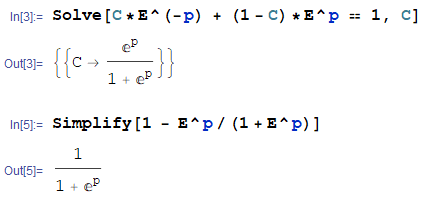
\includegraphics[scale=0.5]{1.png}
			\end{figure}
			\begin{figure}[h!]
				\centering
				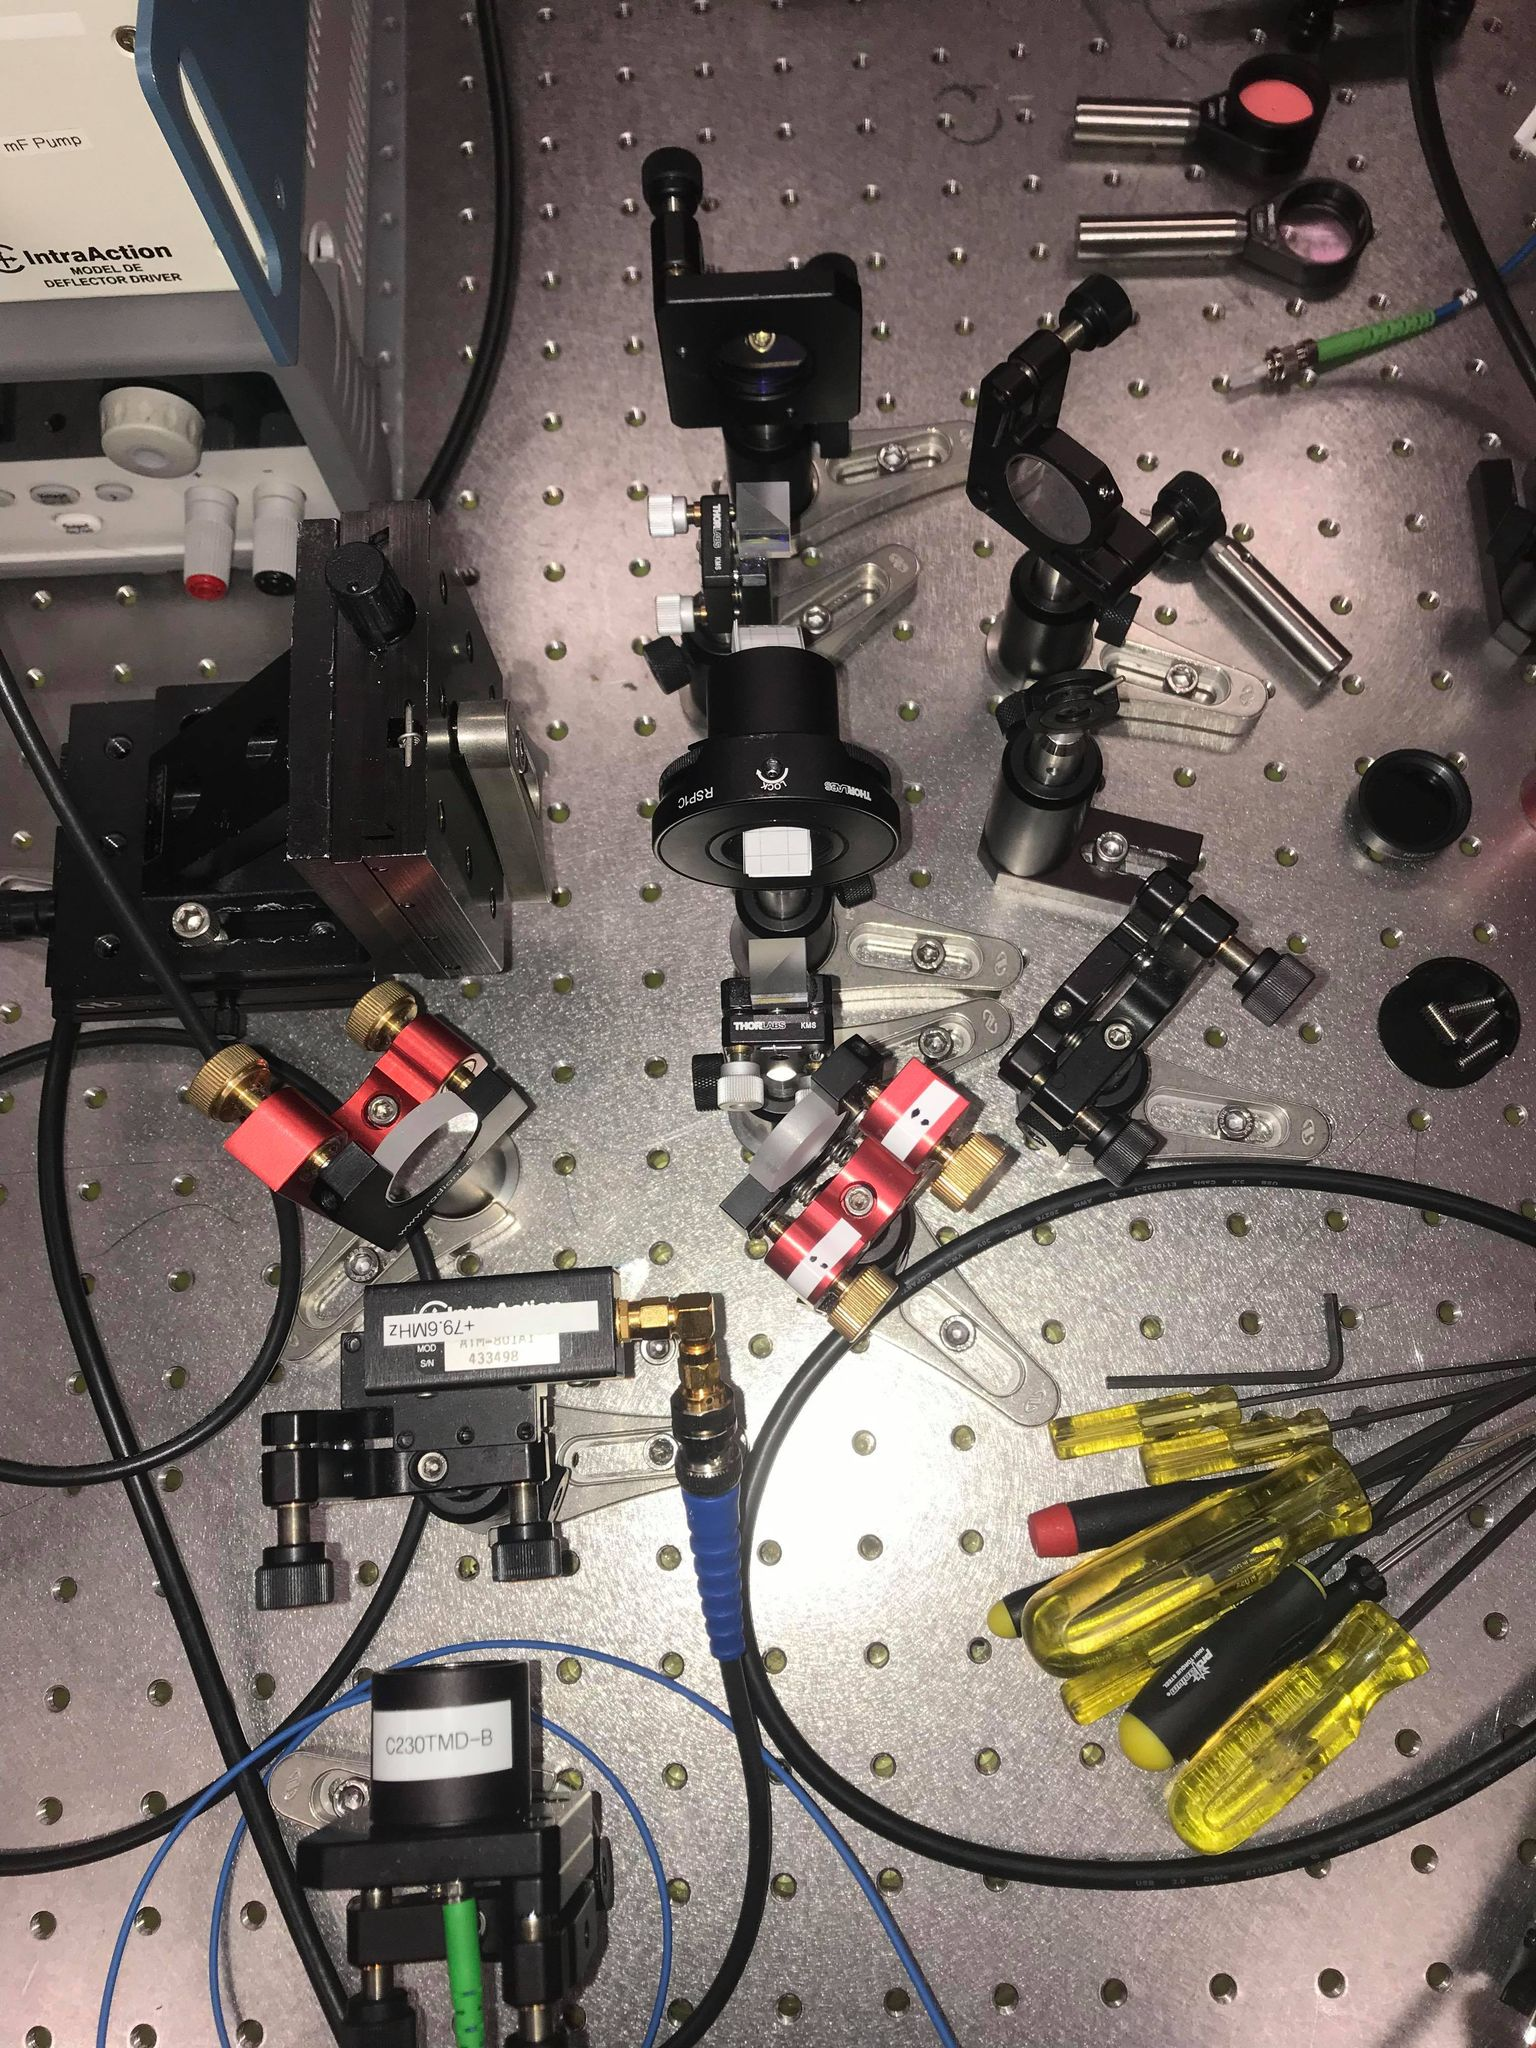
\includegraphics[scale=0.5]{2.png}
			\end{figure}
		\end{sln*}
	\end{prob*}
\end{exer}

\newpage


\begin{exer}
	\begin{prob*}1, Lesson 3. Sketch the solution to the IBVP (Farlow, 3.6) for different values of time. Check if they agree with the boundary conditions. What is the steady-state temperature of the rod? Is this obvious?\\
		
		The IBVP:
		\begin{align*}
		\begin{cases}
		PDE: u_t = \alpha^2 u_{xx}, x\in(0,200), t\in(0,\infty)\\
		BC_1: u_x(0,t) = 0, t\in(0,\infty)\\
		BC_2: u_x(200,t) = -\frac{h}{k}[u(200,t) - 20], t\in(0,\infty)\\
		IC: u(x,0) = 0, x\in[0,200]
		\end{cases}
		\end{align*}
		\begin{sln}
			Sketches:\\\\\\\\\\\\\\\\\\\\\\\\\\\\\\\\\\\\\\\\\\\\\\\\\\\\\\\\
			
			Intuitively, the steady-state temperature of the rod is just 20$^\circ$C, since the rod in the problem, which is initially at 0$^\circ$C, is simply being warmed up by the 20$^\circ$C water. We can of course show this mathematically. By the steady-state condition, $u_t = 0 = u_{xx}$. This forces $u_{xx} = Cx + D$. But by the first boundary condition $u_x(0,t)=0$, require that $C = 0$. The second boundary condition requires that $u_{s,x} = C = 0 = (-h/k)[u(200,t) -20] = (-h/k)[200C + D - 20]$, which means $D=20$. So, the steady-state temperature profile, not surprisingly, is 20$^\circ$C uniform along the length of the rod. 
		\end{sln}
	\end{prob*}
	\newpage
	\begin{prob*}2, Lesson 3. Interpret the IBVP:
		\begin{align*}
		\begin{cases}
		PDE: u_t = \alpha^2 u_{xx}, x\in(0,1), t\in(0,\infty)\\
		BC_1: u(0,t) = 0, t\in(0,\infty)\\
		BC_2: u_x(1,t) = 1, t\in(0,\infty)\\
		IC: u(x,0) = \sin(\pi x), x\in[0,1]
		\end{cases}
		\end{align*}
		\begin{sln}
			$\,$\\
			
			\textit{Interpretation:} The PDE suggests that we are dealing with heat flow in one dimension, so we can imagine a rod of length 1 with no laterally heat transfer. The first boundary condition suggests that the temperature is held fixed at 0 at $x=0$ for all $t$. The second boundary condition suggests that temperature is increasing (at a constant rate) at $x=1$ end. The initial condition tells us that initially, the temperature profile of the rod has a sinusoidal distribution across the rod's length, with the ends having temperature of 0 ($\sin(0)=\sin(\pi) = 0$) and the middle $x=1/2$ having the highest temperature of 1. \\
			
			\textit{Steady-state?} The steady-state condition requires that $u_{xx} = 0$, so again, we have $u_s(x) = Cx +D$, where $C,D$ are real constants. The first boundary condition requires $D=0$. The second boundary condition requires that $u_x(1) = C\times 1 = C = 1$. Therefore, in the long run, $u_s(x) = x$. So, the stead-state temperature at each point of the rod has the same value as the position (from the 0 degree end) of that point on the rod. \\
			
			\textit{Sketches:}
		\end{sln}
	\end{prob*}
	\newpage
	\begin{prob*}3, Lesson 3. Interpret the following IBVP:
		\begin{align*}
		\begin{cases}
		PDE: u_t = \alpha^2 u_{xx}, x\in(0,1), t\in(0,\infty)\\
		BC_1: u_x(0,t) = 0, t\in(0,\infty)\\
		BC_2: u_x(1,t) = 0, t\in(0,\infty)\\
		IC: u(x,0) = \sin(\pi x), x\in[0,1]
		\end{cases}
		\end{align*}
		\begin{sln}
			$\,$\\
			
			\textit{Interpretation:} The PDE suggests that we are dealing with heat flow in one dimension, so we can imagine a rod of length 1 with no laterally heat transfer. The boundary conditions suggest that there are no temperature gradients at the ends of the rod. So we imagine the rod being insulated at the ends. The initial condition is like that in the previous problem where the temperature profile of the rod has a sinusoidal distribution across the rod's length, with the ends being at zero degrees ($\sin(0)=\sin(\pi) = 0$) and the middle $x=1/2$ having the highest temperature of 1. \\
			
			\textit{Steady-state:} The steady-state condition requires that $u_{xx} = 0$, i.e., $u_s(x) = Cx + D$, where $C,D$ are real constants. Since the temperatures are fixed at the end points, $u_{s,x} = C = 0$. So the steady state temperature is $D$, which takes some value between 0 and 1 as $t\to \infty$. The steady-state temperature profile is the same along the length of the rod. \\
			
			\textit{Sketches:}
		\end{sln}
	\end{prob*}
\end{exer}

\newpage


\begin{exer}
	\begin{prob*}3, Lesson 4. Derive the heat equation
		\begin{align*}
		u_t = \frac{1}{c\rho}\p_x[k(x)u_x] + f(x,t)
		\end{align*}
		for the situation where the thermal conductivity $k(x)$ depends on $x$.\\
		\begin{sln*}
			We can start the derivation from step (4.2) in Farlow's, modify $k \to k(x)$. The conservation of energy gives:
			\begin{align*}
			c\rho A\int_{x}^{x+\Delta x}u_t(s,t)\,ds = A\left(k(x+\Delta x)u_x(x+\Delta x,t) - k(x)u_x(x,t)  + \int_x^{x+\Delta x}f(s,t)\,ds \right).
			\end{align*}
			By the MVT, there exists $\zeta \in (x,x+\Delta x)$ such that
			\begin{align*}
			c\rho u_t(\zeta, t)\Delta x = k(x+\Delta x)u_x(x+\Delta x,t) - k(x)u_x(x,t) + f(\zeta,t)\Delta x,
			\end{align*} 
			i.e.,
			\begin{align*}
			u_t(\zeta,t) &= \frac{1}{c\rho}\left\{ \frac{k(x+\Delta x)u_x(x+\Delta x,t) - k(x)u_x(x,t)}{\Delta x} \right\} + \frac{1}{c\rho}f(\zeta,t)
			\end{align*}
			Letting $\Delta x \to 0$, we turn the term with $\Delta x$ into a derivative of a composition defined as $UK(x,t) = k(x)u_x(x,t)$. The result is
			\begin{align*}
			u_t(x,t) = \frac{1}{c\rho}\p_x(k(x)u_x(x,t)) + f(x,t),
			\end{align*}
			where we simply let $f(x,t)$ absorb the constant $(c\rho)^{-1}$. We have obtained the heat equation with $x$-dependent thermal conductivity. 
		\end{sln*}
	\end{prob*}
\end{exer}

\newpage

\begin{exer}
	\begin{prob*}1, Lesson 5. Show that
		\begin{align*}
		u(x,t) = e^{-\lambda^2\alpha^2 t}(A\sin\lambda x + B\cos \lambda x)
		\end{align*}
		satisfies the PDE $u_t = \alpha^2 u_{xx}$ for $A,B,\lambda \in \R$.
		\begin{sln*}
			We can compute the partial derivatives and verify that $u(x,t)$ solves the PDE ``by inspection.'' The $t$-derivative gives the same $u(x,t)$, multiplied by a factor of $-\lambda^2\alpha^2$, while the $x$-second derivative also gives $u(x,t)$, but multiplied by factor of $\lambda^2$. So, these expressions differ by a factor of $\alpha^2$.  Mathematically:
			\begin{align*}
			u_t = -\lambda^2 \alpha^2 u(x,t) = \alpha^2 u_{xx}.
			\end{align*}
			Hence, $u(x,t)$ solves the given PDE. 
		\end{sln*}
	\end{prob*}
	\newpage
	\begin{prob*}2, Lesson 5. Let $\delta^m_n$ denotes the Kronecker delta, where $m,n$ are non-negative whole numbers. Show
		\begin{align*}
		\int_{0}^{1}\sin(\pi mx)\sin(\pi nx)\,dx = \frac{1}{2}\delta^m_n
		\end{align*}
		\begin{sln*}
			Applying the hinted trigonometric identity, we have
			\begin{align*}
			\int_{0}^{1}\sin(\pi mx)\sin(\pi nx)\,dx &= \frac{1}{2}\int_0^1\cos[(m-n)\pi x] - \cos[(m+n)\pi x]\,dx\\
			&= \frac{1}{2}\int_0^1\cos[(m-n)\pi x]\,dx - \frac{1}{2}\int_0^1\cos[(m+n)\pi x]\,dx
			\end{align*}
			At this point, we can argue why the equality given by the problem is true without much computation. The argument goes as follows. If $m = n$, then the second integral vanishes because $\cos(xk\pi)$, where $k$ is an even number and $x\in [0,1]$, is symmetric about $x=1/2$ and $y=0$. If $m\neq n$, then $m-n$ and $m+n$ are either odd or even. If they are even (and positive), then both integrals on the right hand side vanish. If they are odd, then we can assume (without loss of generality) that $m$ is odd and $n$ is even. This makes $\sin(\pi m x)\sin(\pi n x)$ symmetric about $x=1/2$ and $y=0$, so the integral also vanishes over $x\in[0,1]$.
		\end{sln*}
	\end{prob*}
	\newpage
	\begin{prob*}5, Lesson 5. What is the solution to problem 4 in Farlow, Lesson 5 (which also requires doing 3) if the initial condition is changed to 
		\begin{align*}
		u(x,0) = \sin(2\pi x) + \frac{1}{3}\sin(4\pi x) + \frac{1}{5}\sin(6\pi x)
		\end{align*}
		\begin{sln*}
			We should quickly do problem 3 first. If $\Phi(x) = 1$, $x\in[0,1]$. Applying the formula for the coefficients $A_n$:
			\begin{align*}
			A_n = 2\int_0^1\Phi(x)\sin(n\pi x)\,dx = 2\int_0^1\sin(n\pi x)\,dx = \frac{2}{n\pi}(1-\cos(n\pi x)) = \begin{cases}
			\frac{4}{n\pi}, n \text{ odd}\\
			0, n\text{ even}
			\end{cases}.
			\end{align*}
			So, the Fourier expansion for $\Phi(x) = 1$ is
			\begin{align*}
			\Phi(x) =1 = \frac{4}{\pi}\left[\sin(\pi x) + \frac{1}{3}\sin(3\pi x) + \frac{1}{5}\sin(5\pi x)+\dots \right].
			\end{align*}
			In problem 4, the boundary and initial conditions suggests using $\Phi(x)$ from problem 3. So, given the formula for $u(x,t)$, we simply substitute in the coefficients to generate a Fourier expansion for $u(x,t)$:
			\begin{align*}
			u(x,t) &= \sum_{n=1}^{\infty}A_n e^{-(n\pi)^2t}\sin(n\pi x)\\
			&= \frac{4}{\pi}\left[ e^{-(\pi)^2t}\sin(\pi x) + \frac{1}{3}e^{-(3\pi)^2t}\sin(3\pi x)
			+ \frac{1}{5}e^{-(5\pi)^2t}\sin(5\pi x)+\dots\right].
			\end{align*}
			Back to problem 5, if the initial condition is given as $u(x,0)$ above, then we might think we have to re-do and find a new Fourier expansion. But by inspecting the form of $u(x,0)$, we can see that it is just a truncated Fourier expansion. So there is no need to find the coefficients $A_n$ since they are already given to us. So, carefully picking out the coefficients, we get the new solution
			\begin{align*}
			u(x,t) = e^{-(2\pi)^2t}\sin(2\pi x) + \frac{1}{3}e^{-(4\pi)^2t}\sin(4\pi x) + \frac{1}{5}e^{-(6\pi)^2t}\sin(6\pi x).
			\end{align*}
		\end{sln*}
	\end{prob*}
\end{exer}

\newpage
\subsection{Problem set 2}


\begin{exer*}\textbf{Problem 2, Lesson 6}
	
	\noindent Transform
	\begin{align*}
	&PDE: u_t = u_{xx},\,\,\,\,\,\,\,\,\,\,\, 0<x<1\\
	&BCs:  
	\begin{cases}
	u(0,t) = 0\\
	u(1,t) = 1
	\end{cases} 0 < t < \infty\\
	&IC: u(x,0) = x^2,\,\,\,\,\,\,\,\,\,\,\, 0 \leq x\leq 1
	\end{align*}
	to zero BCs and solve the new problem. What will the solution to this problem look like for different values of time? Does the solution agree with your intuition? What is the steady-state solution? What does the transient solution look like?
	\begin{sln*}
		$\,$\\
		Let $u(x,t) = U(x,t) + S(x,t)$ where $U(x,t)$ is the transient solution while $S(x,t)$ is the steady-state solution to the IBVP. To find the steady-state solution $S(x,t)$, we set $u_t = 0$ and $U(x,t) = 0$. Applying the boundary conditions, we find 
		\begin{align*}
		S(x,t) = S(x) = Cx+D = x.
		\end{align*}
		So,
		\begin{align*}
		u(x,t) = x + U(x,t).
		\end{align*}
		Since $u_t = U_t$ and $u_{xx} = U_{xx}$, we can re-write the origin IBVP as
		\begin{align*}
		&PDE: U_t = U_{xx},\,\,\,\,\,\,\,\,\,\,\, 0<x<1\\
		&BCs:  
		\begin{cases}
		U(0,t) = 0\\
		U(1,t) = 0
		\end{cases} 0 < t < \infty\\
		&IC: U(x,0) = x^2 - x,\,\,\,\,\,\,\,\,\,\,\, 0 \leq x\leq 1
		\end{align*}
		The solution $U(x,t)$ to this IBVP is given by
		\begin{align*}
		U(x,t) = \sum^\infty_{n=1}A_n e^{-(n\pi)^2t} \sin(n\pi x),
		\end{align*}
		where
		\begin{align*}
		A_n = 2\int_{0}^{1}(x^2 - x)\sin(n\pi x)\,dx &= \frac{-2+2\cos(n\pi) + n\pi\sin(n\pi)}{n^3\pi^3}\\
		&= \begin{cases}
		\frac{4}{n^3\pi^3},\,\,\,\,\, n \text{ odd}\\
		0,\,\,\,\,\,\,\,\,\, n \text{ even}.
		\end{cases}.
		\end{align*}
		The second equality comes from integrating in Mathematica, which can also be done with integration by parts. The transient solution is then
		\begin{align*}
		U(x,t) = -\frac{4}{\pi ^3}e^{-(\pi)^2t} \sin(\pi x)   -\frac{4}{27 \pi ^3}e^{-(3\pi)^2t} \sin(3\pi x)    -\frac{4}{125 \pi ^3}e^{-(5\pi)^2t} \sin(5\pi x)  + \dots
		\end{align*}
		The full solution to the IBVP is
		\begin{align*}
		u(x,t) &= x- \frac{4}{\pi^3}\sum_{n=1}^\infty\frac{1}{n^3}e^{-(n\pi)^2t}\sin(n\pi x) \\ 
		&= x -\frac{4}{\pi ^3}e^{-(\pi)^2t} \sin(\pi x)   -\frac{4}{27 \pi ^3}e^{-(3\pi)^2t} \sin(3\pi x)    -\frac{4}{125 \pi ^3}e^{-(5\pi)^2t} \sin(5\pi x)  + \dots
		\end{align*}
		
		
		\noindent Mathematica code:
		\begin{lstlisting}
		In[6]:= Simplify[Integrate[(x^2 - x) Sin[n*Pi*x], {x, 0, 1}]]
		
		Out[6]= (-2 + 2 Cos[n \[Pi]] + n \[Pi] Sin[n \[Pi]])/(n^3 \[Pi]^3)
		
		In[4]:= F[n_] := Simplify[Integrate[(x^2 - x) Sin[n*Pi*x], {x, 0, 1}]]
		
		In[7]:= Table[F[n], {n, 1, 10}]
		
		Out[7]= {-(4/\[Pi]^3), 0, -(4/(27 \[Pi]^3)), 0, -(4/(
		125 \[Pi]^3)), 0, -(4/(343 \[Pi]^3)), 0, -(4/(729 \[Pi]^3)), 0}
		\end{lstlisting}
		$\,$\\
		\noindent Solutions for different values of time:\\
		
		\begin{figure}[h!]
			\centering
			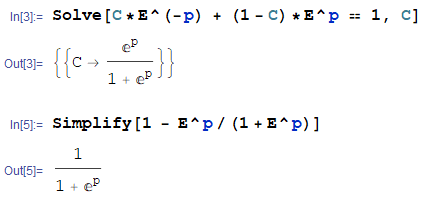
\includegraphics[scale=0.7]{1.png}
		\end{figure}
		
		\noindent Mathematica code:
		\begin{lstlisting}
		U[x_, t_] := 
		x - (4 E^(-\[Pi]^2 t) Sin[\[Pi] x])/\[Pi]^3 - (
		4 E^(-9 \[Pi]^2 t) Sin[3 \[Pi] x])/(27 \[Pi]^3) - (
		4 E^(-25 \[Pi]^2 t) Sin[5 \[Pi] x])/(125 \[Pi]^3)
		
		Show[Plot[U[x, 0], {x, 0, 1}], Plot[U[x, 0.1], {x, 0, 1}], 
		Plot[U[x, 1], {x, 0, 1}]]
		\end{lstlisting}
		
		The solution matches my intuition. The IBVP simply states that the temperature at the ends are fixed, and that the temperature is initially distributed across the rod as $x^2$. Since the temperatures at the ends are fixed it is expected that in the long run the temperature increases uniformly across the rod, in agreement with the steady-state solution. 
		
	\end{sln*}
\end{exer*}
\newpage






\begin{exer*}\textbf{Problem 3, Lesson 6}
	Transform
	\begin{align*}
	&PDE: u_t = u_{xx},\,\,\,\,\,\,\,\,\,\,\, 0<x<1\\
	&BCs:  
	\begin{cases}
	u_x(0,t) = 0\\
	u_x(1,t) + hu(1,t)= 1
	\end{cases} 0 < t < \infty\\
	&IC: u(x,0) = \sin(\pi x),\,\,\,\,\,\,\,\,\,\,\, 0 \leq x\leq 1
	\end{align*}
	into a new problem with zero BCs. Is the new PDE homogeneous?
	
	\begin{sln*}
		$\,$\\
		Once again, we let $u(x,t) = U(x,t) + S(x,t)$ where $S(x,t)$ is the steady-state solution. $S(x,t)$ has the form:
		\begin{align*}
		S(x,t) = A(t)\left( 1 - \frac{x}{L} \right) + B(t)\left( \frac{x}{L} \right) = A(t)\left( 1 - x \right) + B(t)\left( x \right),
		\end{align*} 
		where
		\begin{align*}
		S(0,t) &= A(t)\\
		S(1,t) &= B(t)\\
		S_x(0,t) &= B(t) - A(t) = S_x(1,t).
		\end{align*}
		Applying the boundary conditions,
		\begin{align*}
		\begin{pmatrix}
		-1 & 1\\
		-1 & h + 1
		\end{pmatrix}
		\begin{pmatrix}
		A(t) \\ B(t)
		\end{pmatrix}
		=
		\begin{pmatrix}
		0\\1
		\end{pmatrix}
		\end{align*} 
		Solving the system for $A(t)$ and $B(t)$ gives
		\begin{align*}
		A(t) = B(t) = \frac{1}{h}
		\end{align*}
		So, the steady-state solution is
		\begin{align*}
		S(x,t) = \frac{1}{h}(1-x+x) = \frac{1}{h},
		\end{align*}
		which is independent of $t$ and $x$. Therefore, $u_t = U_t = u_{xx} = U_{xx}$. Applying the initial condition, we find 
		\begin{align*}
		u(x,0) = S(x,0) + U(x,0) = \frac{1}{h} + U(x,0) = \sin(\pi x)
		\end{align*}
		and
		\begin{align*}
		u_x(1,t) + hu(1,t) = U(1,t) + hU(1,t) + \frac{h}{h} = 1.
		\end{align*}
		So, the new IBVP is:
		\begin{align*}
		&PDE: U_t = U_{xx},\,\,\,\,\,\,\,\,\,\,\, 0<x<1\\
		&BCs:  
		\begin{cases}
		U_x(0,t) = 0\\
		U_x(1,t) + hU(1,t)= 0
		\end{cases} 0 < t < \infty\\
		&IC: u(x,0) = \sin(\pi x)-\frac{1}{h}   ,\,\,\,\,\,\,\,\,\,\,\, 0 \leq x\leq 1
		\end{align*}
		We notice that the new PDE is still homogeneous. 
	\end{sln*}
\end{exer*}
\newpage









\begin{exer*}\textbf{Problem 1, Lesson 7}
	Solve the following heat-flaw problem:
	\begin{align*}
	&PDE: u_t = u_{xx},\,\,\,\,\,\,\,\,\,\,\, 0<x<1, 0<t<\infty\\
	&BCs:  
	\begin{cases}
	u(0,t) = 0\\
	u_x(1,t) = 0
	\end{cases} 0 < t < \infty\\
	&IC: u(x,0) = x,\,\,\,\,\,\,\,\,\,\,\, 0 \leq x\leq 1
	\end{align*}
	by separation of variables. Does your solution agree with the your intuition? What is the steady-state solution? 
	\begin{sln*}
		$\,$\\
		
		\noindent By separation of variables, we assume $u(x,t) = T(t)X(x)$. By the PDE, 
		\begin{align*}
		\frac{T'(t)}{T(t)} = \frac{X''(x)}{X(x)} = \mu,
		\end{align*}
		where $\mu$ is some constant. We reject solutions with $\mu > 0$ on physical grounds. If $\mu = 0$, then $T'(t) = X''(x) = 0$, so
		\begin{align*}
		u(x,t) = Ax + B.
		\end{align*}
		To satisfy the boundary conditions:
		\begin{align*}
		u(0,t) &= B = 0\\
		u_x(1,t) &= A = 0.
		\end{align*}
		This $u(x,t) = 0$, a trivial solution. If $\mu < 0$, then we let $\mu = -\lambda^2$. We immediately have
		\begin{align*}
		T(t) &= Ae^{-\lambda^2 t}\\
		X(x) &= C\sin(\lambda x) + B\cos(\lambda x).
		\end{align*}
		So, the general solution is
		\begin{align*}
		u(x,t) = e^{-\lambda^2 t}(A\sin(\lambda x) + B\cos(\lambda x)).
		\end{align*}
		Subjecting $u(x,t)$ to the first boundary condition, we find $B = 0$, which reduces the solution to
		\begin{align*}
		u(x,t) = Ae^{-\lambda^2 t}\sin(\lambda x).
		\end{align*}
		The second boundary condition gives
		\begin{align*}
		A\cos(\lambda)= 0.
		\end{align*}
		Assuming $A\neq 0$, so that our solution is not trivial, 
		\begin{align*}
		\lambda = k\pi,\,\,\,\,\,\,\,\, k\in \mathbb{Z}.
		\end{align*}
		The solution is then
		\begin{align*}
		u(x,t) = \sum_{k=1}^{\infty}A_ke^{-(k\pi)^2t}\sin(k\pi x).
		\end{align*}
		To find the coefficients $A_k$, we invoke Fourier's trick:
		\begin{align*}
		\int_{0}^1 u_0(x)\sin(n\pi x)\,dx &= \int_0^1 \sin(n\pi x)\sum_{k=1}^\infty A_k\sin(k\pi x)\,dx\\
		&= \sum_{k=1}^\infty A_k \int_{0}^1 \sin(n\pi x)\sin(k\pi x)\,dx\\
		&= \sum_{k=1}^\infty \frac{1}{2}A_k\delta^k_n\\
		&= \frac{1}{2}A_n.
		\end{align*}
		Integration by parts gives
		\begin{align*}
		A_k = 2\int_{0}^1x\sin(k\pi x)\,dx = \frac{2\sin (\pi  k)-2\pi  k \cos (\pi  k)}{\pi ^2 k^2} = \frac{2(-1)^{k+1}}{k\pi}.
		\end{align*}
		So, the transient solution has the form:
		\begin{align*}
		U(x,t) &= \sum_{k=1}^\infty A_k e^{-(k\pi)^2t} \sin(k\pi x)\\
		&= \frac{2}{\pi }e^{-(\pi)^2t}\sin(\pi x) -\frac{1}{\pi }e^{-(2\pi)^2t} \sin(2\pi x) + \frac{2}{3 \pi }e^{-(3\pi)^2t} \sin(3\pi x)-\frac{1}{2 \pi }e^{-(4\pi)^2t} \sin(4\pi x) + \dots
		\end{align*}
		The full solution is then
		\begin{align*}
		u(x,t) &= \frac{1}{h} + \frac{2}{\pi}\sum_{n=1}^\infty \frac{(-1)^{k+1}}{k}e^{-(k\pi)^2t} \sin(k\pi x)\\
		&= \frac{1}{h} + \frac{2}{\pi }e^{-(\pi)^2t}\sin(\pi x) -\frac{1}{\pi }e^{-(2\pi)^2t} \sin(2\pi x) + \frac{2}{3 \pi }e^{-(3\pi)^2t} \sin(3\pi x)-\frac{1}{2 \pi }e^{-(4\pi)^2t} \sin(4\pi x) + \dots
		\end{align*}
		
		\noindent Mathematica code:\\
		\begin{lstlisting}
		Integrate[Sin[k*Pi*x], {x, 0, 1}]
		(1 - Cos[k \[Pi]])/(k \[Pi])
		
		Simplify[2*Integrate[x*Sin[k*Pi*x], {x, 0, 1}]]
		(2 (-k \[Pi] Cos[k \[Pi]] + Sin[k \[Pi]]))/(k^2 \[Pi]^2)
		
		F[k_] := (2 (-k \[Pi] Cos[k \[Pi]] + Sin[k \[Pi]]))/(k^2 \[Pi]^2)
		Table[F[k], {k, 1, 4}]
		{2/\[Pi], -(1/\[Pi]), 2/(3 \[Pi]), -(1/(2 \[Pi]))}
		
		u[x_, t_, h_] := 
		1/h + (2 E^(-\[Pi]^2 t) Sin[\[Pi] x])/\[Pi] - (
		E^(-4 \[Pi]^2 t) Sin[2 \[Pi] x])/\[Pi] + (
		2 E^(-9 \[Pi]^2 t) Sin[3 \[Pi] x])/(3 \[Pi]) - (
		E^(-16 \[Pi]^2 t) Sin[4 \[Pi] x])/(2 \[Pi])
		
		Show[Plot[u[x, 0.002, 2], {x, 0, 1}], Plot[u[x, 0.05, 2], {x, 0, 1}], 
		Plot[u[x, 0.1, 2], {x, 0, 1}], Plot[u[x, 0.2, 2], {x, 0, 1}], 
		AxesLabel -> {x, u}]
		\end{lstlisting}
		
		\noindent The figure below shows solutions for different values of time. Here, I'm setting $h=2$, so the steady-state temperature is $u = 0.5$. Notice that $u_0(x)$ is not quite $x$ because I don't have enough terms in the solution.\\
		
		\begin{figure}[h!]
			\centering
			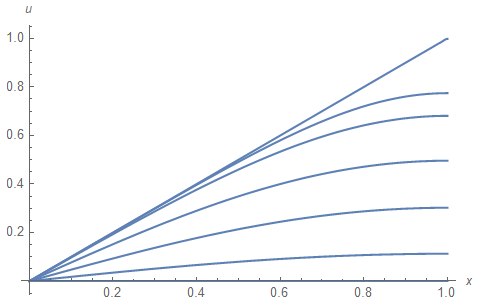
\includegraphics[scale=0.7]{pset2_2.png}
		\end{figure}
		
		\noindent The solution has good sense, first because the steady-state solution is a constant that is equal to $1/h$, as expected. The boundary condition requires the temperature at $x=0$ stay fixed and the temperature gradient at $x=1$ to be zero, which the plot also illustrates. 
	\end{sln*}
	
\end{exer*}
\newpage









\begin{exer*}\textbf{Problem 2, Lesson 7}
	What are the eigenvalues and eigenfunctions of the Sturm-Liouville problem?
	\begin{align*}
	&ODE: X'' + \lambda X = 0,\,\,\,\,\,\,\,\,\,\,\, 0<x<1\\
	&BCs:  
	\begin{cases}
	X(0) = 0\\
	X'(1) = 0
	\end{cases}
	\end{align*}
	What are the functions $p(x)$, $q(x)$, and $r(x)$ in the general Sturm-Liouville problem for this equation? 
	
	\begin{sln*} 
		$\,$
		\begin{enumerate}
			\item $p(x) = 1$.
			\item $q(x) = 0$.
			\item $r(x) = 1$.
		\end{enumerate}
		To find the eigenvalues and the eigenfunctions, we have to solve the IVP. By the ODE, we know that 
		\begin{align*}
		X(t) = A\sin(\sqrt{\lambda}x) + B\cos(\sqrt{\lambda} x).
		\end{align*}
		Applying the initial conditions, we find 
		\begin{align*}
		B = 0\\
		-A\sqrt{\lambda}\cos(\sqrt{\lambda}) = 0.
		\end{align*}
		i.e., for $n$ odd, we find the eigenvalues:
		\begin{align*}
		\lambda_n = \left( \frac{n\pi}{2} \right)^2.
		\end{align*}
		And so the eigenfunctions are
		\begin{align*}
		X_n(t) = A_n\sin\left( \frac{n\pi}{2} \right).
		\end{align*}
	\end{sln*}
\end{exer*}
\newpage









\begin{exer*}\textbf{Problem 3, Lesson 7}
	Solve the following problem with insulated boundaries:
	\begin{align*}
	&PDE: u_t = u_{xx},\,\,\,\,\,\,\,\,\,\,\, 0<x<1, 0<t<\infty\\
	&BCs:  
	\begin{cases}
	u_x(0,t) = 0\\
	u_x(1,t) = 0
	\end{cases} 0 < t < \infty\\
	&IC: u(x,0) = x,\,\,\,\,\,\,\,\,\,\,\, 0 \leq x\leq 1
	\end{align*}
	Does your solution agree with your interpretation of the problem? What is the steady-state solution? Does this make sense? 
	\begin{sln*}
		$\,$\\
		\noindent Let $u(x,t) = U(x,t) + S(x,t)$ where $S(x,t)$ is the steady-state and $U(x,t)$ is the transient solution. We can construct the steady-state solution as
		\begin{align*}
		S(x,t) = A(t)\left(1 -x \right) + B(t)x.
		\end{align*}
		As before, by applying the boundary conditions, we require that $A(t)$ and $B(t)$ solve the following linear system
		\begin{align*}
		\begin{pmatrix}
		-1 & 1\\
		-1 & 1
		\end{pmatrix}
		\begin{pmatrix}
		A(t) \\ B(t)
		\end{pmatrix}
		=
		\begin{pmatrix}
		0\\0
		\end{pmatrix}.
		\end{align*}
		The system has infinitely many solutions, but we get $A(t) = B(t)$. Assuming that at steady-state, $u_t = u_{xx} = 0 = S_t$, we get
		\begin{align*}
		S(x,t) = A(t)(1-x) + A(t)x = A(t) = \Lambda
		\end{align*}
		where $\Lambda$ is constant. Applying separation of variables to this PDE, we know that 
		\begin{align*}
		T(t) = e^{-\lambda^2 t}\\
		X_n(x) = A\cos(\lambda x)  + B\sin(\lambda x).
		\end{align*}
		Applying the boundary conditions, 
		\begin{align*}
		B&= 0\\
		\lambda_n &= n\pi.
		\end{align*}
		So, the general solution is
		\begin{align*}
		u(x,t) = \Lambda + \sum_{n=1}^\infty A_n e^{-(n\pi)^2 t}\cos(n\pi x).
		\end{align*}
		Next, we want to find the coefficients $A_n$. Since there is a $\cos$ involved, we will use Fourier's trick with a cosine and the identity
		\begin{align*}
		\int_{0}^1\cos(m\pi x)\cos(n\pi x) = \frac{1}{2}\delta^m_n.
		\end{align*}
		This gives
		\begin{align*}
		\int_{0}^1 u_0(x)\cos(m\pi x)\,dx &= \int_{0}^1 \cos(m\pi x)\sum_{n=1}^\infty A_n \cos(n\pi x)\,dx\\
		&= \sum_{n=1}^\infty A_n \frac{1}{2}\delta^n_m\\
		&= \frac{A_m}{2}.
		\end{align*}
		So, we can compute $A_m$ in Mathematica (or by integration by parts):
		\begin{align*}
		A_m = 2\int_{0}^1 x\cos(m\pi x)\,dx &= \frac{2 (\pi  m \sin (\pi  m)+\cos (\pi  m)-1)}{\pi ^2 m^2}\\
		&= \frac{2(\cos(\pi m - 1))}{m^2\pi^2}\\
		&= \begin{cases}
		\frac{4}{m^2\pi^2},\,\,\,\,\,\, m \text{ odd}\\
		0,\,\,\,\,\,\,\,\, m \text{ even}.
		\end{cases}
		\end{align*}
		The general solution is then
		\begin{align*}
		u(x,t) &= \Lambda + \frac{4}{\pi^2}\sum_{n=1}^\infty \frac{1}{n^2}\cos(n\pi x)\\
		&= \Lambda -\frac{4}{\pi ^2}e^{-(\pi)^2 t}\cos(\pi x)    -\frac{4}{9 \pi ^2}e^{-(3\pi)^2 t}\cos(3\pi x)        -\frac{4}{25 \pi ^2}e^{-(5\pi)^2 t}\cos(5\pi x) + \dots
		\end{align*}
		
		\noindent Mathematica code:
		\begin{lstlisting}
		Simplify[Integrate[Cos[m*Pi*x]*Cos[n*Pi*x], {x, 0, 1}]]
		(m Cos[n \[Pi]] Sin[m \[Pi]] - n Cos[m \[Pi]] Sin[n \[Pi]])/(
		m^2 \[Pi] - n^2 \[Pi])
		
		2*Integrate[x*Cos[m*Pi*x], {x, 0, 1}]
		(2 (-1 + Cos[m \[Pi]] + m \[Pi] Sin[m \[Pi]]))/(m^2 \[Pi]^2)
		
		A[m_] := (2 (-1 + Cos[m \[Pi]] + m \[Pi] Sin[m \[Pi]]))/(m^2 \[Pi]^2)
		Table[A[m], {m, 1, 7}]
		{-(4/\[Pi]^2), 0, -(4/(9 \[Pi]^2)), 0, -(4/(25 \[Pi]^2)), 0, -(4/(
		49 \[Pi]^2))}
		\end{lstlisting}
	\end{sln*}
\end{exer*}


\newpage
\subsection{Problem set 3}

\newpage
\subsection{Problem set 4}





























\end{document}
